% Seminar 7: Efficient markets, random walk and variance-ratio tests
% Statistics of Financial Markets -- Bachelor's programme, Bucharest University of Economic Studies
% GENERATED by latex/build_seminar7.py -- edit the generator, not this file.
% Student version by default; the instructor version is the *_solutions.tex wrapper.
\makeatletter\@ifundefined{ifsolutions}{\expandafter\newif\csname ifsolutions\endcsname}{}\makeatother

\newcommand{\coursename}{Statistics of Financial Markets}
% Preambul comun SFM -- Statistica piețelor financiare / Statistics of Financial Markets (Beamer, 16:9)
% Același design ca MFM. Înainte de % Preambul comun SFM -- Statistica piețelor financiare / Statistics of Financial Markets (Beamer, 16:9)
% Același design ca MFM. Înainte de % Preambul comun SFM -- Statistica piețelor financiare / Statistics of Financial Markets (Beamer, 16:9)
% Același design ca MFM. Înainte de \input{../../latex/preamble} se definește
%   \newcommand{\coursename}{Statistics of Financial Markets}      (EN)
%   \newcommand{\coursename}{Statistica piețelor financiare}       (RO)  și  \def\sfmlang{ro}
% Fișierele .tex se află în EN/Courses, EN/Seminars, RO/Cursuri, RO/Seminarii (două niveluri sub rădăcină).
% Deck-urile sînt generate de latex/build_chapterN.py / build_seminarN.py (vezi latex/sfm_build.py).

\documentclass[9pt, aspectratio=169, t]{beamer}
\providecommand{\coursename}{Statistics of Financial Markets}

% Ensure content fits on slides
\setbeamersize{text margin left=8mm, text margin right=8mm}

%=============================================================================
% THEME AND STYLE CONFIGURATION
%=============================================================================
\usetheme{default}
% Using default theme for clean header/footer control

% Color Palette (matching Redispatch PDF)
\definecolor{MainBlue}{RGB}{26, 58, 110}
\definecolor{AccentBlue}{RGB}{26, 58, 110}
\definecolor{IDAred}{RGB}{205, 0, 0}
\definecolor{DarkGray}{RGB}{51, 51, 51}
\definecolor{MediumGray}{RGB}{128, 128, 128}
\definecolor{LightGray}{RGB}{248, 248, 248}
\definecolor{VeryLightGray}{RGB}{235, 235, 235}
\definecolor{KeynoteGray}{RGB}{218, 218, 218}
\definecolor{SectionGray}{RGB}{120, 120, 120}
\definecolor{FooterGray}{RGB}{100, 100, 100}
\definecolor{Crimson}{RGB}{220, 53, 69}
\definecolor{Forest}{RGB}{46, 125, 50}
\definecolor{Amber}{RGB}{181, 133, 63}
\definecolor{Orange}{RGB}{230, 126, 34}
\definecolor{Purple}{RGB}{142, 68, 173}

% Gradient background (exact Keynote 315° gradient: white to RGB 218,218,218)
\setbeamertemplate{background}{%
    \begin{tikzpicture}[remember picture, overlay]
        \shade[shading=axis, shading angle=315,
        top color=white, bottom color=KeynoteGray]
        (current page.south west) rectangle (current page.north east);
    \end{tikzpicture}%
}
% Fallback solid color for compatibility
\setbeamercolor{background canvas}{bg=}

\setbeamercolor{palette primary}{bg=MainBlue, fg=white}
\setbeamercolor{palette secondary}{bg=MainBlue!85, fg=white}
\setbeamercolor{palette tertiary}{bg=MainBlue!70, fg=white}
\setbeamercolor{structure}{fg=MainBlue}
\setbeamercolor{title}{fg=IDAred}
\setbeamercolor{frametitle}{fg=IDAred, bg=}
\setbeamercolor{block title}{bg=MainBlue, fg=white}
\setbeamercolor{block body}{bg=VeryLightGray, fg=DarkGray}
\setbeamercolor{block title alerted}{bg=Crimson, fg=white}
\setbeamercolor{block body alerted}{bg=Crimson!8, fg=DarkGray}
\setbeamercolor{block title example}{bg=Forest, fg=white}
\setbeamercolor{block body example}{bg=Forest!8, fg=DarkGray}
\setbeamercolor{item}{fg=MainBlue}

% Footer colors (override Madrid theme blue)
\setbeamercolor{author in head/foot}{fg=FooterGray, bg=}
\setbeamercolor{title in head/foot}{fg=FooterGray, bg=}
\setbeamercolor{date in head/foot}{fg=FooterGray, bg=}
\setbeamercolor{section in head/foot}{fg=FooterGray, bg=}
\setbeamercolor{subsection in head/foot}{fg=FooterGray, bg=}

% Bullet styles (apply everywhere including blocks)
\setbeamertemplate{itemize item}{\color{MainBlue}$\boxdot$}
\setbeamertemplate{itemize subitem}{\color{MainBlue}$\blacktriangleright$}
\setbeamertemplate{itemize subsubitem}{\color{MainBlue}\tiny$\bullet$}
\setbeamertemplate{itemize/enumerate body begin}{\normalsize}
\setbeamertemplate{itemize/enumerate subbody begin}{\normalsize}

% Item spacing - compact style
\setlength{\leftmargini}{10pt}       % Level 1: minimal indent
\setlength{\leftmarginii}{10pt}      % Level 2: minimal additional indent
% Compact list spacing (zero extra space before/after lists in blocks)
\makeatletter
\def\@listi{\leftmargin\leftmargini \topsep 0pt \parsep 0pt \itemsep 0pt}
\def\@listii{\leftmargin\leftmarginii \topsep 0pt \parsep 0pt \itemsep 0pt}
\makeatother

\setbeamertemplate{navigation symbols}{}

%=============================================================================
% CUSTOM HEADLINE
%=============================================================================
\setbeamertemplate{headline}{%
    \vskip10pt%
    \hbox to \paperwidth{%
        \hskip0.5cm%
        {\small\color{FooterGray}\renewcommand{\hyperlink}[2]{##2}\insertsectionhead}%
        \hfill%
        \textcolor{FooterGray}{\small\insertframenumber}%
        \hskip0.5cm%
    }%
    \vskip4pt%
    {\color{FooterGray}\hrule height 0.4pt}%
}

%=============================================================================
% CUSTOM FOOTER
%=============================================================================
\usepackage{fontawesome5}

\setbeamertemplate{footline}{%
    {\color{FooterGray}\hrule height 0.4pt}%
    \vskip4pt%
    \hbox to \paperwidth{%
        \hskip0.5cm%
        \textcolor{FooterGray}{\small\coursename}%
        \hfill%
        \raisebox{-0.1em}{%
            \begin{tikzpicture}[x=0.08em, y=0.08em, line width=0.4pt]
                \draw[FooterGray] (0,3) -- (1,4) -- (2,3.5) -- (3,5) -- (4,4) -- (5,6) -- (6,5.5) -- (7,4) -- (8,5) -- (9,7) -- (10,6) -- (11,5) -- (12,6.5) -- (13,8) -- (14,7) -- (15,6) -- (16,7.5) -- (17,9) -- (18,8) -- (19,7) -- (20,8.5) -- (21,10) -- (22,9) -- (23,8) -- (24,9.5);
            \end{tikzpicture}%
        }%
        \hskip0.5cm%
    }%
    \vskip6pt%
}

%=============================================================================
% PACKAGES
%=============================================================================
\usepackage[utf8]{inputenc}
\DeclareUnicodeCharacter{03B1}{\ensuremath{\alpha}}
\usepackage[T1]{fontenc}
\usepackage{amsmath, amssymb, amsthm}
\usepackage{mathtools}
\usepackage{bm}
\usepackage{tikz}
\usetikzlibrary{arrows.meta, positioning, shapes, calc, decorations.pathreplacing, shadings}
\usepackage{booktabs}
\usepackage{multirow}
\usepackage{array}
\usepackage{graphicx}
\usepackage{hyperref}
\usepackage{colortbl}
\usepackage{listings}
\lstset{language=Python, basicstyle=\ttfamily\scriptsize, keywordstyle=\color{MainBlue}\bfseries,
  commentstyle=\color{Forest}, stringstyle=\color{Crimson}, breaklines=true,
  frame=none, backgroundcolor=\color{VeryLightGray}, xleftmargin=2mm}
\hypersetup{colorlinks=true, linkcolor=MainBlue, urlcolor=MainBlue}
\graphicspath{{../../logos/}{../../charts/}{../../photos/}}
\usepackage{xcolor}
\hfuzz=2pt  % Suppress tiny overfull warnings (<2pt)
\vfuzz=2pt  % Suppress tiny vertical overfull warnings (<2pt)

%=============================================================================
% QUANTLET COMMANDS
%   \quantlet{<displayed name>}{<url>}       (generic, compatible with the older SFM decks)
%   \sfmquantlet{Ch_05}{SFM_ch5_garch}       -> https://github.com/danpele/SFM/tree/main/Quantlets/Ch_05/SFM_ch5_garch
%   \qlurl{<folder>} is defined per chapter by the generator (Quantlets/Ch_NN/<folder>)
%=============================================================================
\newcommand{\sfmrepo}{https://github.com/danpele/SFM}
\newcommand{\sfmqlbase}{https://github.com/danpele/SFM/tree/main/Quantlets}
\newcommand{\quantlet}[2]{%
    \hfill\href{#2}{%
        \raisebox{-0.15em}{
\includegraphics[height=0.7em]{ql_logo.png}}%
        \textcolor{MainBlue}{\tiny\ #1}%
    }%
}
\newcommand{\sfmquantlet}[2]{\quantlet{\detokenize{#2}}{\sfmqlbase/#1/#2}}

%=============================================================================
% NOTEBOOKS (Google Colab)
%   \colaburl{notebooks/EN/chapter5_seminar_notebook.ipynb} -> the Colab link of a file in the SFM repo
%   \nb: the chapter notebook (each seminar deck redefines it with \renewcommand)
%=============================================================================
\newcommand{\colaburl}[1]{https://colab.research.google.com/github/danpele/SFM/blob/main/#1}
\newcommand{\nb}{https://colab.research.google.com/github/danpele/SFM/tree/main/notebooks/EN}
\newcommand{\nbname}{notebooks/EN}

%=============================================================================
% SLIDE HELPERS (used by the generators; the same as in MFM)
%=============================================================================
% local font size for list bodies (the preamble forces \normalsize)
\newcommand{\itemsize}[1]{\setbeamertemplate{itemize/enumerate body begin}{#1}\setbeamertemplate{itemize/enumerate subbody begin}{#1}}
\newcommand{\intitle}[1]{{\hypersetup{urlcolor=white}#1}}   % white links inside coloured title bars
\newcommand{\imgcap}[1]{{\scriptsize #1}\\[0.5mm]}          % caption under a photo
\newcommand{\imgcredit}[2]{{\tiny\color{FooterGray}\href{#1}{#2}}}   % image credit: source URL, author/licence
\newcommand{\aiprompt}[1]{{\ttfamily\color{MainBlue}#1}}     % a prompt to an AI assistant

%=============================================================================
% SEMINARS: student version by default; the instructor wrapper *_solutions.tex sets \solutionstrue
%=============================================================================
\makeatletter\@ifundefined{ifsolutions}{\expandafter\newif\csname ifsolutions\endcsname}{}\makeatother
\newcommand{\solonly}[1]{\ifsolutions #1\fi}
\newcommand{\propsub}{\ifsolutions\else\framesubtitle{\ifdefined\sfmlang Rezolvarea se discută la seminar\else Solution discussed in class\fi}\fi}

%=============================================================================
% APPENDIX AND CHAPTER LINKS (latex/appendix_links.py writes the calls; it also re-declares these
% macros before \begin{document}, so the decks compile with or without this preamble block)
%=============================================================================
\providecommand{\sfmapplink}[3]{\hypertarget{#2}{}\hyperlink{#1}{\beamergotobutton{#3}}}
\providecommand{\sfmappback}[2]{\begin{tikzpicture}[remember picture,overlay]\node[anchor=south east] at ([xshift=-3mm,yshift=7mm]current page.south east){\hyperlink{#1}{\beamerreturnbutton{#2}}};\end{tikzpicture}}
\providecommand{\sfmchlink}[2]{\href{#1}{#2}}
\providecommand{\sfmchlinkt}[2]{\href{#1}{\usebeamercolor[fg]{frametitle}#2}}

%=============================================================================
% QUANTINAR COMMAND: link către un curs Quantinar (subiecte avansate)
%=============================================================================
\newcommand{\quantinar}[2]{%
    \href{#2}{%
        \raisebox{-0.15em}{
\includegraphics[height=0.8em]{qr_logo.png}}%
        \textcolor{MainBlue}{\scriptsize\ #1}%
    }%
}

%=============================================================================
% CUSTOM TITLE PAGE
%=============================================================================
\defbeamertemplate*{title page}{hybrid}[1][]
{
    \vspace{0.2cm}
    % Logos row - top header (with clickable links)
    \begin{center}
        \href{https://www.ase.ro}{
\includegraphics[height=1.0cm]{ase_logo.png}}\hspace{0.3cm}%
        \href{https://theida.net}{
\includegraphics[height=1.0cm]{ida_logo.png}}\hspace{0.3cm}%
        \href{https://blockchain-research-center.com}{
\includegraphics[height=1.0cm]{brc_logo.png}}\hspace{0.3cm}%
        \href{https://www.ai4efin.ase.ro}{
\includegraphics[height=1.0cm]{ai4efin_logo.png}}\hspace{0.3cm}%
        \href{https://ipe.ro/new}{
\includegraphics[height=1.0cm]{acad_logo.png}}\hspace{0.3cm}%
        \href{https://www.digital-finance-msca.com}{
\includegraphics[height=1.0cm]{msca_logo.png}}%
    \end{center}

    \vspace{0.6cm}

    % Main title with Q logos on sides (with clickable links)
    \begin{center}
        \begin{minipage}{0.1\textwidth}
            \centering
            \href{https://quantlet.com}{
\includegraphics[height=1.1cm]{ql_logo.png}}
        \end{minipage}%
        \begin{minipage}{0.78\textwidth}
            \centering
            {\LARGE\bfseries\usebeamercolor[fg]{title}\inserttitle}

            \vspace{0.3cm}

            {\usebeamerfont{subtitle}\usebeamercolor[fg]{title}\insertsubtitle}
        \end{minipage}%
        \begin{minipage}{0.1\textwidth}
            \centering
            \href{https://quantinar.com}{
\includegraphics[height=1.1cm]{qr_logo.png}}
        \end{minipage}
    \end{center}

    \vspace{0.6cm}

    % Authors (left aligned)
    \hspace{0.5cm}{\usebeamerfont{author}\insertauthor}

    \vspace{0.3cm}

    % Institute/Affiliations (left aligned)
    \hspace{0.5cm}\begin{minipage}[t]{0.9\textwidth}
        \raggedright\small\insertinstitute
    \end{minipage}
}

%=============================================================================
% THEOREM ENVIRONMENTS
%=============================================================================
\theoremstyle{definition}
\setbeamertemplate{theorems}[numbered]
\ifdefined\sfmlang
\newtheorem{defn}{Definiție}
\newtheorem{thm}{Teoremă}
\newtheorem{prop}{Propoziție}
\newtheorem{rmk}{Observație}
\else
\newtheorem{defn}{Definition}
\newtheorem{thm}{Theorem}
\newtheorem{prop}{Proposition}
\newtheorem{rmk}{Remark}
\fi

%=============================================================================
% CENTRED MINIPAGE (no extra vertical space)
%=============================================================================
\newenvironment{cminipage}[1]{%
    \par\noindent\hfill\begin{minipage}{#1}\ignorespaces
}{%
    \end{minipage}\hfill\null\par
}

%=============================================================================
% CUSTOM COMMANDS
%=============================================================================
\newcommand{\E}{\mathbb{E}}
\newcommand{\Var}{\text{Var}}
\newcommand{\Cov}{\text{Cov}}
\newcommand{\Corr}{\text{Corr}}
\newcommand{\R}{\mathbb{R}}
\newcommand{\N}{\mathbb{N}}
\newcommand{\Z}{\mathbb{Z}}
\newcommand{\B}{\mathbf{B}}
\newcommand{\imark}{\textcolor{MainBlue}{\textbullet}}
\newcommand{\RMSE}{\text{RMSE}}
\newcommand{\MAE}{\text{MAE}}
\newcommand{\MAPE}{\text{MAPE}}

 se definește
%   \newcommand{\coursename}{Statistics of Financial Markets}      (EN)
%   \newcommand{\coursename}{Statistica piețelor financiare}       (RO)  și  \def\sfmlang{ro}
% Fișierele .tex se află în EN/Courses, EN/Seminars, RO/Cursuri, RO/Seminarii (două niveluri sub rădăcină).
% Deck-urile sînt generate de latex/build_chapterN.py / build_seminarN.py (vezi latex/sfm_build.py).

\documentclass[9pt, aspectratio=169, t]{beamer}
\providecommand{\coursename}{Statistics of Financial Markets}

% Ensure content fits on slides
\setbeamersize{text margin left=8mm, text margin right=8mm}

%=============================================================================
% THEME AND STYLE CONFIGURATION
%=============================================================================
\usetheme{default}
% Using default theme for clean header/footer control

% Color Palette (matching Redispatch PDF)
\definecolor{MainBlue}{RGB}{26, 58, 110}
\definecolor{AccentBlue}{RGB}{26, 58, 110}
\definecolor{IDAred}{RGB}{205, 0, 0}
\definecolor{DarkGray}{RGB}{51, 51, 51}
\definecolor{MediumGray}{RGB}{128, 128, 128}
\definecolor{LightGray}{RGB}{248, 248, 248}
\definecolor{VeryLightGray}{RGB}{235, 235, 235}
\definecolor{KeynoteGray}{RGB}{218, 218, 218}
\definecolor{SectionGray}{RGB}{120, 120, 120}
\definecolor{FooterGray}{RGB}{100, 100, 100}
\definecolor{Crimson}{RGB}{220, 53, 69}
\definecolor{Forest}{RGB}{46, 125, 50}
\definecolor{Amber}{RGB}{181, 133, 63}
\definecolor{Orange}{RGB}{230, 126, 34}
\definecolor{Purple}{RGB}{142, 68, 173}

% Gradient background (exact Keynote 315° gradient: white to RGB 218,218,218)
\setbeamertemplate{background}{%
    \begin{tikzpicture}[remember picture, overlay]
        \shade[shading=axis, shading angle=315,
        top color=white, bottom color=KeynoteGray]
        (current page.south west) rectangle (current page.north east);
    \end{tikzpicture}%
}
% Fallback solid color for compatibility
\setbeamercolor{background canvas}{bg=}

\setbeamercolor{palette primary}{bg=MainBlue, fg=white}
\setbeamercolor{palette secondary}{bg=MainBlue!85, fg=white}
\setbeamercolor{palette tertiary}{bg=MainBlue!70, fg=white}
\setbeamercolor{structure}{fg=MainBlue}
\setbeamercolor{title}{fg=IDAred}
\setbeamercolor{frametitle}{fg=IDAred, bg=}
\setbeamercolor{block title}{bg=MainBlue, fg=white}
\setbeamercolor{block body}{bg=VeryLightGray, fg=DarkGray}
\setbeamercolor{block title alerted}{bg=Crimson, fg=white}
\setbeamercolor{block body alerted}{bg=Crimson!8, fg=DarkGray}
\setbeamercolor{block title example}{bg=Forest, fg=white}
\setbeamercolor{block body example}{bg=Forest!8, fg=DarkGray}
\setbeamercolor{item}{fg=MainBlue}

% Footer colors (override Madrid theme blue)
\setbeamercolor{author in head/foot}{fg=FooterGray, bg=}
\setbeamercolor{title in head/foot}{fg=FooterGray, bg=}
\setbeamercolor{date in head/foot}{fg=FooterGray, bg=}
\setbeamercolor{section in head/foot}{fg=FooterGray, bg=}
\setbeamercolor{subsection in head/foot}{fg=FooterGray, bg=}

% Bullet styles (apply everywhere including blocks)
\setbeamertemplate{itemize item}{\color{MainBlue}$\boxdot$}
\setbeamertemplate{itemize subitem}{\color{MainBlue}$\blacktriangleright$}
\setbeamertemplate{itemize subsubitem}{\color{MainBlue}\tiny$\bullet$}
\setbeamertemplate{itemize/enumerate body begin}{\normalsize}
\setbeamertemplate{itemize/enumerate subbody begin}{\normalsize}

% Item spacing - compact style
\setlength{\leftmargini}{10pt}       % Level 1: minimal indent
\setlength{\leftmarginii}{10pt}      % Level 2: minimal additional indent
% Compact list spacing (zero extra space before/after lists in blocks)
\makeatletter
\def\@listi{\leftmargin\leftmargini \topsep 0pt \parsep 0pt \itemsep 0pt}
\def\@listii{\leftmargin\leftmarginii \topsep 0pt \parsep 0pt \itemsep 0pt}
\makeatother

\setbeamertemplate{navigation symbols}{}

%=============================================================================
% CUSTOM HEADLINE
%=============================================================================
\setbeamertemplate{headline}{%
    \vskip10pt%
    \hbox to \paperwidth{%
        \hskip0.5cm%
        {\small\color{FooterGray}\renewcommand{\hyperlink}[2]{##2}\insertsectionhead}%
        \hfill%
        \textcolor{FooterGray}{\small\insertframenumber}%
        \hskip0.5cm%
    }%
    \vskip4pt%
    {\color{FooterGray}\hrule height 0.4pt}%
}

%=============================================================================
% CUSTOM FOOTER
%=============================================================================
\usepackage{fontawesome5}

\setbeamertemplate{footline}{%
    {\color{FooterGray}\hrule height 0.4pt}%
    \vskip4pt%
    \hbox to \paperwidth{%
        \hskip0.5cm%
        \textcolor{FooterGray}{\small\coursename}%
        \hfill%
        \raisebox{-0.1em}{%
            \begin{tikzpicture}[x=0.08em, y=0.08em, line width=0.4pt]
                \draw[FooterGray] (0,3) -- (1,4) -- (2,3.5) -- (3,5) -- (4,4) -- (5,6) -- (6,5.5) -- (7,4) -- (8,5) -- (9,7) -- (10,6) -- (11,5) -- (12,6.5) -- (13,8) -- (14,7) -- (15,6) -- (16,7.5) -- (17,9) -- (18,8) -- (19,7) -- (20,8.5) -- (21,10) -- (22,9) -- (23,8) -- (24,9.5);
            \end{tikzpicture}%
        }%
        \hskip0.5cm%
    }%
    \vskip6pt%
}

%=============================================================================
% PACKAGES
%=============================================================================
\usepackage[utf8]{inputenc}
\DeclareUnicodeCharacter{03B1}{\ensuremath{\alpha}}
\usepackage[T1]{fontenc}
\usepackage{amsmath, amssymb, amsthm}
\usepackage{mathtools}
\usepackage{bm}
\usepackage{tikz}
\usetikzlibrary{arrows.meta, positioning, shapes, calc, decorations.pathreplacing, shadings}
\usepackage{booktabs}
\usepackage{multirow}
\usepackage{array}
\usepackage{graphicx}
\usepackage{hyperref}
\usepackage{colortbl}
\usepackage{listings}
\lstset{language=Python, basicstyle=\ttfamily\scriptsize, keywordstyle=\color{MainBlue}\bfseries,
  commentstyle=\color{Forest}, stringstyle=\color{Crimson}, breaklines=true,
  frame=none, backgroundcolor=\color{VeryLightGray}, xleftmargin=2mm}
\hypersetup{colorlinks=true, linkcolor=MainBlue, urlcolor=MainBlue}
\graphicspath{{../../logos/}{../../charts/}{../../photos/}}
\usepackage{xcolor}
\hfuzz=2pt  % Suppress tiny overfull warnings (<2pt)
\vfuzz=2pt  % Suppress tiny vertical overfull warnings (<2pt)

%=============================================================================
% QUANTLET COMMANDS
%   \quantlet{<displayed name>}{<url>}       (generic, compatible with the older SFM decks)
%   \sfmquantlet{Ch_05}{SFM_ch5_garch}       -> https://github.com/danpele/SFM/tree/main/Quantlets/Ch_05/SFM_ch5_garch
%   \qlurl{<folder>} is defined per chapter by the generator (Quantlets/Ch_NN/<folder>)
%=============================================================================
\newcommand{\sfmrepo}{https://github.com/danpele/SFM}
\newcommand{\sfmqlbase}{https://github.com/danpele/SFM/tree/main/Quantlets}
\newcommand{\quantlet}[2]{%
    \hfill\href{#2}{%
        \raisebox{-0.15em}{
\includegraphics[height=0.7em]{ql_logo.png}}%
        \textcolor{MainBlue}{\tiny\ #1}%
    }%
}
\newcommand{\sfmquantlet}[2]{\quantlet{\detokenize{#2}}{\sfmqlbase/#1/#2}}

%=============================================================================
% NOTEBOOKS (Google Colab)
%   \colaburl{notebooks/EN/chapter5_seminar_notebook.ipynb} -> the Colab link of a file in the SFM repo
%   \nb: the chapter notebook (each seminar deck redefines it with \renewcommand)
%=============================================================================
\newcommand{\colaburl}[1]{https://colab.research.google.com/github/danpele/SFM/blob/main/#1}
\newcommand{\nb}{https://colab.research.google.com/github/danpele/SFM/tree/main/notebooks/EN}
\newcommand{\nbname}{notebooks/EN}

%=============================================================================
% SLIDE HELPERS (used by the generators; the same as in MFM)
%=============================================================================
% local font size for list bodies (the preamble forces \normalsize)
\newcommand{\itemsize}[1]{\setbeamertemplate{itemize/enumerate body begin}{#1}\setbeamertemplate{itemize/enumerate subbody begin}{#1}}
\newcommand{\intitle}[1]{{\hypersetup{urlcolor=white}#1}}   % white links inside coloured title bars
\newcommand{\imgcap}[1]{{\scriptsize #1}\\[0.5mm]}          % caption under a photo
\newcommand{\imgcredit}[2]{{\tiny\color{FooterGray}\href{#1}{#2}}}   % image credit: source URL, author/licence
\newcommand{\aiprompt}[1]{{\ttfamily\color{MainBlue}#1}}     % a prompt to an AI assistant

%=============================================================================
% SEMINARS: student version by default; the instructor wrapper *_solutions.tex sets \solutionstrue
%=============================================================================
\makeatletter\@ifundefined{ifsolutions}{\expandafter\newif\csname ifsolutions\endcsname}{}\makeatother
\newcommand{\solonly}[1]{\ifsolutions #1\fi}
\newcommand{\propsub}{\ifsolutions\else\framesubtitle{\ifdefined\sfmlang Rezolvarea se discută la seminar\else Solution discussed in class\fi}\fi}

%=============================================================================
% APPENDIX AND CHAPTER LINKS (latex/appendix_links.py writes the calls; it also re-declares these
% macros before \begin{document}, so the decks compile with or without this preamble block)
%=============================================================================
\providecommand{\sfmapplink}[3]{\hypertarget{#2}{}\hyperlink{#1}{\beamergotobutton{#3}}}
\providecommand{\sfmappback}[2]{\begin{tikzpicture}[remember picture,overlay]\node[anchor=south east] at ([xshift=-3mm,yshift=7mm]current page.south east){\hyperlink{#1}{\beamerreturnbutton{#2}}};\end{tikzpicture}}
\providecommand{\sfmchlink}[2]{\href{#1}{#2}}
\providecommand{\sfmchlinkt}[2]{\href{#1}{\usebeamercolor[fg]{frametitle}#2}}

%=============================================================================
% QUANTINAR COMMAND: link către un curs Quantinar (subiecte avansate)
%=============================================================================
\newcommand{\quantinar}[2]{%
    \href{#2}{%
        \raisebox{-0.15em}{
\includegraphics[height=0.8em]{qr_logo.png}}%
        \textcolor{MainBlue}{\scriptsize\ #1}%
    }%
}

%=============================================================================
% CUSTOM TITLE PAGE
%=============================================================================
\defbeamertemplate*{title page}{hybrid}[1][]
{
    \vspace{0.2cm}
    % Logos row - top header (with clickable links)
    \begin{center}
        \href{https://www.ase.ro}{
\includegraphics[height=1.0cm]{ase_logo.png}}\hspace{0.3cm}%
        \href{https://theida.net}{
\includegraphics[height=1.0cm]{ida_logo.png}}\hspace{0.3cm}%
        \href{https://blockchain-research-center.com}{
\includegraphics[height=1.0cm]{brc_logo.png}}\hspace{0.3cm}%
        \href{https://www.ai4efin.ase.ro}{
\includegraphics[height=1.0cm]{ai4efin_logo.png}}\hspace{0.3cm}%
        \href{https://ipe.ro/new}{
\includegraphics[height=1.0cm]{acad_logo.png}}\hspace{0.3cm}%
        \href{https://www.digital-finance-msca.com}{
\includegraphics[height=1.0cm]{msca_logo.png}}%
    \end{center}

    \vspace{0.6cm}

    % Main title with Q logos on sides (with clickable links)
    \begin{center}
        \begin{minipage}{0.1\textwidth}
            \centering
            \href{https://quantlet.com}{
\includegraphics[height=1.1cm]{ql_logo.png}}
        \end{minipage}%
        \begin{minipage}{0.78\textwidth}
            \centering
            {\LARGE\bfseries\usebeamercolor[fg]{title}\inserttitle}

            \vspace{0.3cm}

            {\usebeamerfont{subtitle}\usebeamercolor[fg]{title}\insertsubtitle}
        \end{minipage}%
        \begin{minipage}{0.1\textwidth}
            \centering
            \href{https://quantinar.com}{
\includegraphics[height=1.1cm]{qr_logo.png}}
        \end{minipage}
    \end{center}

    \vspace{0.6cm}

    % Authors (left aligned)
    \hspace{0.5cm}{\usebeamerfont{author}\insertauthor}

    \vspace{0.3cm}

    % Institute/Affiliations (left aligned)
    \hspace{0.5cm}\begin{minipage}[t]{0.9\textwidth}
        \raggedright\small\insertinstitute
    \end{minipage}
}

%=============================================================================
% THEOREM ENVIRONMENTS
%=============================================================================
\theoremstyle{definition}
\setbeamertemplate{theorems}[numbered]
\ifdefined\sfmlang
\newtheorem{defn}{Definiție}
\newtheorem{thm}{Teoremă}
\newtheorem{prop}{Propoziție}
\newtheorem{rmk}{Observație}
\else
\newtheorem{defn}{Definition}
\newtheorem{thm}{Theorem}
\newtheorem{prop}{Proposition}
\newtheorem{rmk}{Remark}
\fi

%=============================================================================
% CENTRED MINIPAGE (no extra vertical space)
%=============================================================================
\newenvironment{cminipage}[1]{%
    \par\noindent\hfill\begin{minipage}{#1}\ignorespaces
}{%
    \end{minipage}\hfill\null\par
}

%=============================================================================
% CUSTOM COMMANDS
%=============================================================================
\newcommand{\E}{\mathbb{E}}
\newcommand{\Var}{\text{Var}}
\newcommand{\Cov}{\text{Cov}}
\newcommand{\Corr}{\text{Corr}}
\newcommand{\R}{\mathbb{R}}
\newcommand{\N}{\mathbb{N}}
\newcommand{\Z}{\mathbb{Z}}
\newcommand{\B}{\mathbf{B}}
\newcommand{\imark}{\textcolor{MainBlue}{\textbullet}}
\newcommand{\RMSE}{\text{RMSE}}
\newcommand{\MAE}{\text{MAE}}
\newcommand{\MAPE}{\text{MAPE}}

 se definește
%   \newcommand{\coursename}{Statistics of Financial Markets}      (EN)
%   \newcommand{\coursename}{Statistica piețelor financiare}       (RO)  și  \def\sfmlang{ro}
% Fișierele .tex se află în EN/Courses, EN/Seminars, RO/Cursuri, RO/Seminarii (două niveluri sub rădăcină).
% Deck-urile sînt generate de latex/build_chapterN.py / build_seminarN.py (vezi latex/sfm_build.py).

\documentclass[9pt, aspectratio=169, t]{beamer}
\providecommand{\coursename}{Statistics of Financial Markets}

% Ensure content fits on slides
\setbeamersize{text margin left=8mm, text margin right=8mm}

%=============================================================================
% THEME AND STYLE CONFIGURATION
%=============================================================================
\usetheme{default}
% Using default theme for clean header/footer control

% Color Palette (matching Redispatch PDF)
\definecolor{MainBlue}{RGB}{26, 58, 110}
\definecolor{AccentBlue}{RGB}{26, 58, 110}
\definecolor{IDAred}{RGB}{205, 0, 0}
\definecolor{DarkGray}{RGB}{51, 51, 51}
\definecolor{MediumGray}{RGB}{128, 128, 128}
\definecolor{LightGray}{RGB}{248, 248, 248}
\definecolor{VeryLightGray}{RGB}{235, 235, 235}
\definecolor{KeynoteGray}{RGB}{218, 218, 218}
\definecolor{SectionGray}{RGB}{120, 120, 120}
\definecolor{FooterGray}{RGB}{100, 100, 100}
\definecolor{Crimson}{RGB}{220, 53, 69}
\definecolor{Forest}{RGB}{46, 125, 50}
\definecolor{Amber}{RGB}{181, 133, 63}
\definecolor{Orange}{RGB}{230, 126, 34}
\definecolor{Purple}{RGB}{142, 68, 173}

% Gradient background (exact Keynote 315° gradient: white to RGB 218,218,218)
\setbeamertemplate{background}{%
    \begin{tikzpicture}[remember picture, overlay]
        \shade[shading=axis, shading angle=315,
        top color=white, bottom color=KeynoteGray]
        (current page.south west) rectangle (current page.north east);
    \end{tikzpicture}%
}
% Fallback solid color for compatibility
\setbeamercolor{background canvas}{bg=}

\setbeamercolor{palette primary}{bg=MainBlue, fg=white}
\setbeamercolor{palette secondary}{bg=MainBlue!85, fg=white}
\setbeamercolor{palette tertiary}{bg=MainBlue!70, fg=white}
\setbeamercolor{structure}{fg=MainBlue}
\setbeamercolor{title}{fg=IDAred}
\setbeamercolor{frametitle}{fg=IDAred, bg=}
\setbeamercolor{block title}{bg=MainBlue, fg=white}
\setbeamercolor{block body}{bg=VeryLightGray, fg=DarkGray}
\setbeamercolor{block title alerted}{bg=Crimson, fg=white}
\setbeamercolor{block body alerted}{bg=Crimson!8, fg=DarkGray}
\setbeamercolor{block title example}{bg=Forest, fg=white}
\setbeamercolor{block body example}{bg=Forest!8, fg=DarkGray}
\setbeamercolor{item}{fg=MainBlue}

% Footer colors (override Madrid theme blue)
\setbeamercolor{author in head/foot}{fg=FooterGray, bg=}
\setbeamercolor{title in head/foot}{fg=FooterGray, bg=}
\setbeamercolor{date in head/foot}{fg=FooterGray, bg=}
\setbeamercolor{section in head/foot}{fg=FooterGray, bg=}
\setbeamercolor{subsection in head/foot}{fg=FooterGray, bg=}

% Bullet styles (apply everywhere including blocks)
\setbeamertemplate{itemize item}{\color{MainBlue}$\boxdot$}
\setbeamertemplate{itemize subitem}{\color{MainBlue}$\blacktriangleright$}
\setbeamertemplate{itemize subsubitem}{\color{MainBlue}\tiny$\bullet$}
\setbeamertemplate{itemize/enumerate body begin}{\normalsize}
\setbeamertemplate{itemize/enumerate subbody begin}{\normalsize}

% Item spacing - compact style
\setlength{\leftmargini}{10pt}       % Level 1: minimal indent
\setlength{\leftmarginii}{10pt}      % Level 2: minimal additional indent
% Compact list spacing (zero extra space before/after lists in blocks)
\makeatletter
\def\@listi{\leftmargin\leftmargini \topsep 0pt \parsep 0pt \itemsep 0pt}
\def\@listii{\leftmargin\leftmarginii \topsep 0pt \parsep 0pt \itemsep 0pt}
\makeatother

\setbeamertemplate{navigation symbols}{}

%=============================================================================
% CUSTOM HEADLINE
%=============================================================================
\setbeamertemplate{headline}{%
    \vskip10pt%
    \hbox to \paperwidth{%
        \hskip0.5cm%
        {\small\color{FooterGray}\renewcommand{\hyperlink}[2]{##2}\insertsectionhead}%
        \hfill%
        \textcolor{FooterGray}{\small\insertframenumber}%
        \hskip0.5cm%
    }%
    \vskip4pt%
    {\color{FooterGray}\hrule height 0.4pt}%
}

%=============================================================================
% CUSTOM FOOTER
%=============================================================================
\usepackage{fontawesome5}

\setbeamertemplate{footline}{%
    {\color{FooterGray}\hrule height 0.4pt}%
    \vskip4pt%
    \hbox to \paperwidth{%
        \hskip0.5cm%
        \textcolor{FooterGray}{\small\coursename}%
        \hfill%
        \raisebox{-0.1em}{%
            \begin{tikzpicture}[x=0.08em, y=0.08em, line width=0.4pt]
                \draw[FooterGray] (0,3) -- (1,4) -- (2,3.5) -- (3,5) -- (4,4) -- (5,6) -- (6,5.5) -- (7,4) -- (8,5) -- (9,7) -- (10,6) -- (11,5) -- (12,6.5) -- (13,8) -- (14,7) -- (15,6) -- (16,7.5) -- (17,9) -- (18,8) -- (19,7) -- (20,8.5) -- (21,10) -- (22,9) -- (23,8) -- (24,9.5);
            \end{tikzpicture}%
        }%
        \hskip0.5cm%
    }%
    \vskip6pt%
}

%=============================================================================
% PACKAGES
%=============================================================================
\usepackage[utf8]{inputenc}
\DeclareUnicodeCharacter{03B1}{\ensuremath{\alpha}}
\usepackage[T1]{fontenc}
\usepackage{amsmath, amssymb, amsthm}
\usepackage{mathtools}
\usepackage{bm}
\usepackage{tikz}
\usetikzlibrary{arrows.meta, positioning, shapes, calc, decorations.pathreplacing, shadings}
\usepackage{booktabs}
\usepackage{multirow}
\usepackage{array}
\usepackage{graphicx}
\usepackage{hyperref}
\usepackage{colortbl}
\usepackage{listings}
\lstset{language=Python, basicstyle=\ttfamily\scriptsize, keywordstyle=\color{MainBlue}\bfseries,
  commentstyle=\color{Forest}, stringstyle=\color{Crimson}, breaklines=true,
  frame=none, backgroundcolor=\color{VeryLightGray}, xleftmargin=2mm}
\hypersetup{colorlinks=true, linkcolor=MainBlue, urlcolor=MainBlue}
\graphicspath{{../../logos/}{../../charts/}{../../photos/}}
\usepackage{xcolor}
\hfuzz=2pt  % Suppress tiny overfull warnings (<2pt)
\vfuzz=2pt  % Suppress tiny vertical overfull warnings (<2pt)

%=============================================================================
% QUANTLET COMMANDS
%   \quantlet{<displayed name>}{<url>}       (generic, compatible with the older SFM decks)
%   \sfmquantlet{Ch_05}{SFM_ch5_garch}       -> https://github.com/danpele/SFM/tree/main/Quantlets/Ch_05/SFM_ch5_garch
%   \qlurl{<folder>} is defined per chapter by the generator (Quantlets/Ch_NN/<folder>)
%=============================================================================
\newcommand{\sfmrepo}{https://github.com/danpele/SFM}
\newcommand{\sfmqlbase}{https://github.com/danpele/SFM/tree/main/Quantlets}
\newcommand{\quantlet}[2]{%
    \hfill\href{#2}{%
        \raisebox{-0.15em}{
\includegraphics[height=0.7em]{ql_logo.png}}%
        \textcolor{MainBlue}{\tiny\ #1}%
    }%
}
\newcommand{\sfmquantlet}[2]{\quantlet{\detokenize{#2}}{\sfmqlbase/#1/#2}}

%=============================================================================
% NOTEBOOKS (Google Colab)
%   \colaburl{notebooks/EN/chapter5_seminar_notebook.ipynb} -> the Colab link of a file in the SFM repo
%   \nb: the chapter notebook (each seminar deck redefines it with \renewcommand)
%=============================================================================
\newcommand{\colaburl}[1]{https://colab.research.google.com/github/danpele/SFM/blob/main/#1}
\newcommand{\nb}{https://colab.research.google.com/github/danpele/SFM/tree/main/notebooks/EN}
\newcommand{\nbname}{notebooks/EN}

%=============================================================================
% SLIDE HELPERS (used by the generators; the same as in MFM)
%=============================================================================
% local font size for list bodies (the preamble forces \normalsize)
\newcommand{\itemsize}[1]{\setbeamertemplate{itemize/enumerate body begin}{#1}\setbeamertemplate{itemize/enumerate subbody begin}{#1}}
\newcommand{\intitle}[1]{{\hypersetup{urlcolor=white}#1}}   % white links inside coloured title bars
\newcommand{\imgcap}[1]{{\scriptsize #1}\\[0.5mm]}          % caption under a photo
\newcommand{\imgcredit}[2]{{\tiny\color{FooterGray}\href{#1}{#2}}}   % image credit: source URL, author/licence
\newcommand{\aiprompt}[1]{{\ttfamily\color{MainBlue}#1}}     % a prompt to an AI assistant

%=============================================================================
% SEMINARS: student version by default; the instructor wrapper *_solutions.tex sets \solutionstrue
%=============================================================================
\makeatletter\@ifundefined{ifsolutions}{\expandafter\newif\csname ifsolutions\endcsname}{}\makeatother
\newcommand{\solonly}[1]{\ifsolutions #1\fi}
\newcommand{\propsub}{\ifsolutions\else\framesubtitle{\ifdefined\sfmlang Rezolvarea se discută la seminar\else Solution discussed in class\fi}\fi}

%=============================================================================
% APPENDIX AND CHAPTER LINKS (latex/appendix_links.py writes the calls; it also re-declares these
% macros before \begin{document}, so the decks compile with or without this preamble block)
%=============================================================================
\providecommand{\sfmapplink}[3]{\hypertarget{#2}{}\hyperlink{#1}{\beamergotobutton{#3}}}
\providecommand{\sfmappback}[2]{\begin{tikzpicture}[remember picture,overlay]\node[anchor=south east] at ([xshift=-3mm,yshift=7mm]current page.south east){\hyperlink{#1}{\beamerreturnbutton{#2}}};\end{tikzpicture}}
\providecommand{\sfmchlink}[2]{\href{#1}{#2}}
\providecommand{\sfmchlinkt}[2]{\href{#1}{\usebeamercolor[fg]{frametitle}#2}}

%=============================================================================
% QUANTINAR COMMAND: link către un curs Quantinar (subiecte avansate)
%=============================================================================
\newcommand{\quantinar}[2]{%
    \href{#2}{%
        \raisebox{-0.15em}{
\includegraphics[height=0.8em]{qr_logo.png}}%
        \textcolor{MainBlue}{\scriptsize\ #1}%
    }%
}

%=============================================================================
% CUSTOM TITLE PAGE
%=============================================================================
\defbeamertemplate*{title page}{hybrid}[1][]
{
    \vspace{0.2cm}
    % Logos row - top header (with clickable links)
    \begin{center}
        \href{https://www.ase.ro}{
\includegraphics[height=1.0cm]{ase_logo.png}}\hspace{0.3cm}%
        \href{https://theida.net}{
\includegraphics[height=1.0cm]{ida_logo.png}}\hspace{0.3cm}%
        \href{https://blockchain-research-center.com}{
\includegraphics[height=1.0cm]{brc_logo.png}}\hspace{0.3cm}%
        \href{https://www.ai4efin.ase.ro}{
\includegraphics[height=1.0cm]{ai4efin_logo.png}}\hspace{0.3cm}%
        \href{https://ipe.ro/new}{
\includegraphics[height=1.0cm]{acad_logo.png}}\hspace{0.3cm}%
        \href{https://www.digital-finance-msca.com}{
\includegraphics[height=1.0cm]{msca_logo.png}}%
    \end{center}

    \vspace{0.6cm}

    % Main title with Q logos on sides (with clickable links)
    \begin{center}
        \begin{minipage}{0.1\textwidth}
            \centering
            \href{https://quantlet.com}{
\includegraphics[height=1.1cm]{ql_logo.png}}
        \end{minipage}%
        \begin{minipage}{0.78\textwidth}
            \centering
            {\LARGE\bfseries\usebeamercolor[fg]{title}\inserttitle}

            \vspace{0.3cm}

            {\usebeamerfont{subtitle}\usebeamercolor[fg]{title}\insertsubtitle}
        \end{minipage}%
        \begin{minipage}{0.1\textwidth}
            \centering
            \href{https://quantinar.com}{
\includegraphics[height=1.1cm]{qr_logo.png}}
        \end{minipage}
    \end{center}

    \vspace{0.6cm}

    % Authors (left aligned)
    \hspace{0.5cm}{\usebeamerfont{author}\insertauthor}

    \vspace{0.3cm}

    % Institute/Affiliations (left aligned)
    \hspace{0.5cm}\begin{minipage}[t]{0.9\textwidth}
        \raggedright\small\insertinstitute
    \end{minipage}
}

%=============================================================================
% THEOREM ENVIRONMENTS
%=============================================================================
\theoremstyle{definition}
\setbeamertemplate{theorems}[numbered]
\ifdefined\sfmlang
\newtheorem{defn}{Definiție}
\newtheorem{thm}{Teoremă}
\newtheorem{prop}{Propoziție}
\newtheorem{rmk}{Observație}
\else
\newtheorem{defn}{Definition}
\newtheorem{thm}{Theorem}
\newtheorem{prop}{Proposition}
\newtheorem{rmk}{Remark}
\fi

%=============================================================================
% CENTRED MINIPAGE (no extra vertical space)
%=============================================================================
\newenvironment{cminipage}[1]{%
    \par\noindent\hfill\begin{minipage}{#1}\ignorespaces
}{%
    \end{minipage}\hfill\null\par
}

%=============================================================================
% CUSTOM COMMANDS
%=============================================================================
\newcommand{\E}{\mathbb{E}}
\newcommand{\Var}{\text{Var}}
\newcommand{\Cov}{\text{Cov}}
\newcommand{\Corr}{\text{Corr}}
\newcommand{\R}{\mathbb{R}}
\newcommand{\N}{\mathbb{N}}
\newcommand{\Z}{\mathbb{Z}}
\newcommand{\B}{\mathbf{B}}
\newcommand{\imark}{\textcolor{MainBlue}{\textbullet}}
\newcommand{\RMSE}{\text{RMSE}}
\newcommand{\MAE}{\text{MAE}}
\newcommand{\MAPE}{\text{MAPE}}



\newcommand{\qlurl}[1]{https://github.com/danpele/SFM/tree/main/Quantlets/Ch_07/#1}
\renewcommand{\nb}{\colaburl{notebooks/EN/chapter7_seminar_notebook.ipynb}}
\renewcommand{\nbname}{chapter7\_seminar\_notebook.ipynb}
% left column: full width in the student version, narrower next to the solution
\newcommand{\taskw}{\ifsolutions 0.47\textwidth\else 0.96\textwidth\fi}
\newcommand{\solw}{\ifsolutions 0.49\textwidth\else 0pt\fi}

% Clickable citations (DOIs verified via Crossref)

\newcommand{\refFamaA}{\href{https://doi.org/10.1111/j.1540-6261.1970.tb00518.x}{Fama (1970)}}
\newcommand{\refFamaB}{\href{https://doi.org/10.1111/j.1540-6261.1991.tb04636.x}{Fama (1991)}}
\newcommand{\refFamaC}{\href{https://doi.org/10.1086/294743}{Fama (1965)}}
\newcommand{\refSamuelson}{\href{https://doi.org/10.1142/9789814566926_0002}{Samuelson (1965)}}
\newcommand{\refBachelier}{\href{https://doi.org/10.24033/asens.476}{Bachelier (1900)}}
\newcommand{\refKendall}{\href{https://doi.org/10.2307/2980947}{Kendall (1953)}}
\newcommand{\refRoberts}{\href{https://doi.org/10.1111/j.1540-6261.1959.tb00481.x}{Roberts (1959)}}
\newcommand{\refLM}{\href{https://doi.org/10.1093/rfs/1.1.41}{Lo \& MacKinlay (1988)}}
\newcommand{\refLo}{\href{https://doi.org/10.3905/jpm.2004.442611}{Lo (2004)}}
\newcommand{\refLoBook}{\href{https://doi.org/10.1515/9781400887767}{Lo (2017)}}
\newcommand{\refCLM}{\href{https://doi.org/10.1515/9781400830213}{Campbell, Lo \& MacKinlay (1997)}}
\newcommand{\refCD}{\href{https://doi.org/10.1016/0304-4076(93)90051-6}{Chow \& Denning (1993)}}
\newcommand{\refChoi}{\href{https://doi.org/10.1002/(SICI)1099-1255(199905/06)14:3<293::AID-JAE503>3.0.CO;2-5}{Choi (1999)}}
\newcommand{\refKimB}{\href{https://doi.org/10.1016/j.frl.2009.04.003}{Kim (2009)}}
\newcommand{\refAndrews}{\href{https://doi.org/10.2307/2938229}{Andrews (1991)}}
\newcommand{\refLjung}{\href{https://doi.org/10.1093/biomet/65.2.297}{Ljung \& Box (1978)}}
\newcommand{\refBP}{\href{https://doi.org/10.1080/01621459.1970.10481180}{Box \& Pierce (1970)}}
\newcommand{\refWW}{\href{https://doi.org/10.1214/aoms/1177731909}{Wald \& Wolfowitz (1940)}}
\newcommand{\refEL}{\href{https://doi.org/10.1016/j.jeconom.2009.03.001}{Escanciano \& Lobato (2009)}}
\newcommand{\refDF}{\href{https://doi.org/10.1080/01621459.1979.10482531}{Dickey \& Fuller (1979)}}
\newcommand{\refSD}{\href{https://doi.org/10.1093/biomet/71.3.599}{Said \& Dickey (1984)}}
\newcommand{\refPP}{\href{https://doi.org/10.1093/biomet/75.2.335}{Phillips \& Perron (1988)}}
\newcommand{\refKPSS}{\href{https://doi.org/10.1016/0304-4076(92)90104-Y}{Kwiatkowski et al.\ (1992)}}
\newcommand{\refMacKinnon}{\href{https://doi.org/10.1002/(SICI)1099-1255(199611)11:6<601::AID-JAE417>3.0.CO;2-T}{MacKinnon (1996)}}
\newcommand{\refNW}{\href{https://doi.org/10.2307/1913610}{Newey \& West (1987)}}
\newcommand{\refGN}{\href{https://doi.org/10.1016/0304-4076(74)90034-7}{Granger \& Newbold (1974)}}
\newcommand{\refUrquhart}{\href{https://doi.org/10.1016/j.econlet.2016.09.019}{Urquhart (2016)}}
\newcommand{\refUM}{\href{https://doi.org/10.1016/j.irfa.2016.06.011}{Urquhart \& McGroarty (2016)}}
\newcommand{\refKSL}{\href{https://doi.org/10.1016/j.jempfin.2011.08.002}{Kim, Shamsuddin \& Lim (2011)}}
\newcommand{\refLB}{\href{https://doi.org/10.1111/j.1467-6419.2009.00611.x}{Lim \& Brooks (2011)}}
\newcommand{\refGS}{\href{https://ideas.repec.org/a/aea/aecrev/v70y1980i3p393-408.html}{Grossman \& Stiglitz (1980)}}
\newcommand{\refFrench}{\href{https://doi.org/10.1016/0304-405X(80)90021-5}{French (1980)}}
\newcommand{\refRK}{\href{https://doi.org/10.1016/0304-405X(76)90028-3}{Rozeff \& Kinney (1976)}}
\newcommand{\refAriel}{\href{https://doi.org/10.1016/0304-405X(87)90066-3}{Ariel (1987)}}
\newcommand{\refMP}{\href{https://doi.org/10.1111/jofi.12365}{McLean \& Pontiff (2016)}}
\newcommand{\refHLZ}{\href{https://doi.org/10.1093/rfs/hhv059}{Harvey, Liu \& Zhu (2016)}}
\newcommand{\refMacKinlay}{\href{https://ideas.repec.org/a/aea/jeclit/v35y1997i1p13-39.html}{MacKinlay (1997)}}
\newcommand{\refJensen}{\href{https://doi.org/10.1111/j.1540-6261.1968.tb00815.x}{Jensen (1968)}}
\newcommand{\refFF}{\href{https://doi.org/10.1111/j.1540-6261.2010.01598.x}{Fama \& French (2010)}}
\newcommand{\refMalkiel}{\href{https://doi.org/10.1257/089533003321164958}{Malkiel (2003)}}
\newcommand{\refFHH}{\href{https://doi.org/10.1007/978-3-030-13751-9}{Franke, Härdle \& Hafner (2019)}}
\newcommand{\refBHL}{\href{https://doi.org/10.1007/978-3-642-33929-5}{Borak, Härdle \& López-Cabrera (2013)}}
\newcommand{\refTsay}{\href{https://doi.org/10.1002/9780470644560}{Tsay (2010)}}
\newcommand{\refWang}{\href{https://doi.org/10.1038/s41586-023-06221-2}{Wang et al.\ (2023)}}
\newcommand{\refPeleA}{\href{https://doi.org/10.1016/j.sbspro.2012.09.1030}{Pele \& Mazurencu-Marinescu (2012)}}
\newcommand{\refPeleB}{\href{https://doi.org/10.2139/ssrn.7157232}{Tak, Schlamp, Osterrieder \& Pele (2026)}}
\newcommand{\refPeleC}{\href{https://doi.org/10.2139/ssrn.5176758}{Lin, Găman, Wang \& Pele (2025)}}
\newcommand{\refFTSE}{\href{https://www.lseg.com/en/media-centre/press-releases/ftse-russell/2019/ftse-russell-announces-results-country-classification-review-equities-and-fixed-income}{FTSE Russell (2019)}}

\title[Statistics of Financial Markets]{Statistics of Financial Markets}
\subtitle{Seminar 7: Efficient markets, random walk and variance-ratio tests\ifsolutions\ (instructor version)\fi}
\author[D.T. Pele]{Daniel Traian PELE}
\institute{Bucharest University of Economic Studies\\
IDA Institute Digital Assets\\
Blockchain Research Center\\
AI4EFin Artificial Intelligence for Energy Finance\\
Romanian Academy, Institute for Economic Forecasting\\
MSCA Digital Finance}
\date{}

%=============================================================================
\providecommand{\sfmapplink}[3]{\hypertarget{#2}{}\hyperlink{#1}{\beamergotobutton{#3}}}  % APPLINKS-MACROS
\providecommand{\sfmappback}[2]{\begin{tikzpicture}[remember picture,overlay]\node[anchor=south east] at ([xshift=-3mm,yshift=7mm]current page.south east){\hyperlink{#1}{\beamerreturnbutton{#2}}};\end{tikzpicture}}  % APPLINKS-MACROS
\providecommand{\sfmchlink}[2]{\href{#1}{#2}}  % APPLINKS-MACROS
\providecommand{\sfmchlinkt}[2]{\href{#1}{\usebeamercolor[fg]{frametitle}#2}}  % APPLINKS-MACROS
\begin{document}
%=============================================================================

{
\setbeamertemplate{headline}{}
\setbeamertemplate{footline}{}
\begin{frame}[noframenumbering]
    \titlepage
\end{frame}
}
% BEGIN-ACRONYMS (generat de latex/acronyms.py; nu editati manual)
\begin{frame}{Acronyms used in this material}
\setbeamertemplate{itemize/enumerate body begin}{\tiny}
\begin{columns}[T]
\begin{column}{0.49\textwidth}
\begin{itemize}\setlength{\itemsep}{0pt}
    \item \textbf{ACF}: Autocorrelation Function
    \item \textbf{ADF}: Augmented Dickey–Fuller (test)
    \item \textbf{AI}: Artificial Intelligence
    \item \textbf{AIC}: Akaike Information Criterion
    \item \textbf{BET}: Bucharest Exchange Trading (index)
    \item \textbf{BIST}: Borsa İstanbul (BIST 100 index) (the Istanbul Stock Exchange (BIST 100 index))
    \item \textbf{BUX}: Budapesti Értéktőzsde index (the Budapest Stock Exchange index)
    \item \textbf{BVB}: Bursa de Valori București (the Bucharest Stock Exchange)
    \item \textbf{CD}: Chow–Denning (multiple variance-ratio test)
    \item \textbf{COVID-19}: COronaVIrus Disease 2019
    \item \textbf{EODHD}: EOD Historical Data (market-data provider)
    \item \textbf{FTSE}: Financial Times Stock Exchange (FTSE Russell, index provider)
    \item \textbf{KPSS}: Kwiatkowski–Phillips–Schmidt–Shin (stationarity test)
\end{itemize}
\end{column}
\begin{column}{0.49\textwidth}
\begin{itemize}\setlength{\itemsep}{0pt}
    \item \textbf{LB}: Ljung–Box (test)
    \item \textbf{OMV}: Österreichische Mineralölverwaltung (Austrian Mineral Oil Administration (OMV group))
    \item \textbf{PP}: Phillips–Perron (unit-root test)
    \item \textbf{PX}: Prague Stock Exchange index (index Burzy cenných papírů Praha)
    \item \textbf{RW1}: Random Walk 1 (i.i.d. increments)
    \item \textbf{RW2}: Random Walk 2 (independent increments)
    \item \textbf{RW3}: Random Walk 3 (uncorrelated increments)
    \item \textbf{VR}: Variance Ratio
    \item \textbf{WIG20}: Warszawski Indeks Giełdowy 20 (the Warsaw Stock Exchange index of the 20 largest companies)
\end{itemize}
\end{column}
\end{columns}
\end{frame}
% END-ACRONYMS

\begin{frame}{Today's Question and Route}
\itemsize{\small}
\begin{itemize}
    \item \textbf{Question}: how can we test whether past prices predict future returns without fooling ourselves?
    \begin{itemize}
        \item this seminar comes \textbf{before} Lecture 7: the section ``What You Need for Today'' gives every definition the tasks use
    \end{itemize}
    \item Route
    \begin{itemize}
        \item Part A: variance ratios, Ljung--Box statistics, runs and Dickey--Fuller decisions, on paper
        \item Part B: autocorrelation, unit-root and variance-ratio tests on the S\&P 500, DAX, BET, Bitcoin, BVB stocks and emerging markets, each with an interpretation question
        \item Part C: an open question for a project and an AI answer to audit
    \end{itemize}
    \item Notebook for today: \href{\nb}{open the seminar notebook in Google Colab}; each task names its notebook section
    \item The seminar is for practice and is not graded; the solutions of [Proposed] tasks are discussed in class
\end{itemize}
\end{frame}

\begin{frame}{Exercise Map}
\itemsize{\small}
\begin{center}
\footnotesize
\begin{tabular}{>{\raggedright\arraybackslash}p{1.1cm}>{\raggedright\arraybackslash}p{7.5cm}>{\raggedright\arraybackslash}p{1.9cm}>{\raggedright\arraybackslash}p{1.4cm}}
\toprule
\textbf{Task} & \textbf{Question} & \textbf{Type} & \textbf{Model} \\
\midrule
A1, A2 & the square-root-of-time rule and variance ratios from autocorrelations & Solved, Proposed & A1 \\
A3, A4 & Box--Pierce and Ljung--Box statistics, step by step & Solved, Proposed & A3 \\
A5, A6 & the runs test on a sequence of signs & Solved, Proposed & A5 \\
A7, A8 & ADF and KPSS decisions from regression output & Solved, Proposed & A7 \\
B1, B2 & ACF, Ljung--Box and robust tests, runs test: S\&P 500; BET, Bitcoin, BVB stocks & Solved, Proposed & B1 \\
B3, B4 & ADF, Phillips--Perron and KPSS on prices and returns: DAX; BET, Bitcoin, TLV & Solved, Proposed & B3 \\
B5, B6 & variance-ratio tests: S\&P 500; five emerging markets & Solved, Proposed & B5 \\
C1, C2 & has the BET become more efficient? what is wrong in an AI answer? & Proposed & B1, B5 \\
\bottomrule
\end{tabular}
\end{center}
\begin{itemize}
    \item \textbf{[Solved]}: full solution in the slides and in the notebook, a model to follow; \textbf{[Proposed]}: you solve it, following the model
\end{itemize}
\end{frame}

\begin{frame}{Data Used}
\itemsize{\small}
\begin{center}
\footnotesize
\begin{tabular}{llll}
\toprule
\textbf{Series} & \textbf{Source} & \textbf{Price used} & \textbf{Period} \\
\midrule
S\&P 500, DAX & EODHD & close & 1990--2026 \\
BET & EODHD & close & 1997--2026 \\
Bitcoin & EODHD & close, 7 days a week & 2014--2026 \\
Banca Transilvania (TLV), OMV Petrom (SNP) & EODHD & adjusted close & 2010--2026 \\
WIG20, BUX, PX, BIST 100 & EODHD & close & last ten years \\
\bottomrule
\end{tabular}
\end{center}
\begin{itemize}
    \item Daily log returns in \%: $r_t = 100\,(\ln P_t - \ln P_{t-1})$; weekends and repeated holiday closes are dropped (except Bitcoin); the last day is 18 September 2026
    \item TLV: the days 30 and 31 May 2016 are removed (a price adjustment applied one day late, \sfmchlink{https://danpele.github.io/SFM/EN/Courses/chapter2_classical_distributions_stylised_facts.pdf}{Chapter 2})
    \item In the notebook: \texttt{returns('sp500')}, \texttt{log\_price('dax')}; no account or key is needed
\end{itemize}
\end{frame}


%=============================================================================
\section{What You Need for Today}
%=============================================================================

\begin{frame}{What You Need for Today (1/5): Efficiency and Random Walks}
\itemsize{\small}
\begin{itemize}
    \item \textbf{Weak-form efficiency} \refFamaA: past prices cannot be used to earn returns above the return that pays for risk
    \begin{itemize}
        \item excess returns are a \textbf{martingale difference}: $E[r_{t+1} - \mu \mid \text{past}] = 0$
    \end{itemize}
    \item Log price $p_t = \ln P_t$, \textbf{random walk}: $p_t = \mu + p_{t-1} + \varepsilon_t$, so $r_t = \mu + \varepsilon_t$ \refCLM
    \begin{itemize}
        \item \textbf{RW1}: $\varepsilon_t$ i.i.d.\ (independent, identically distributed); \textbf{RW2}: independent; \textbf{RW3}: uncorrelated
        \item RW1 $\Rightarrow$ RW2 $\Rightarrow$ RW3; volatility clustering is allowed only by RW3 and by the martingale
    \end{itemize}
    \item Under any of them, $\mathrm{Var}(r_t(q)) = q\sigma^2$ for the $q$-day return $r_t(q) = r_t + \dots + r_{t-q+1}$
    \begin{itemize}
        \item ``square-root-of-time rule'': $\mathrm{sd}(r_t(q)) = \sigma\sqrt{q}$
    \end{itemize}
\end{itemize}
\end{frame}

\begin{frame}{What You Need for Today (2/5): ACF and Portmanteau Tests}
\itemsize{\small}
\begin{itemize}
    \item Sample \textbf{ACF} (autocorrelation function), with $e_t = r_t - \bar r$: $\hat\rho(k) = \sum_{t>k} e_te_{t-k}\big/\sum_t e_t^2$
    \begin{itemize}
        \item i.i.d.\ returns: $\mathrm{Var}(\hat\rho(k)) \approx 1/T$, 95\% band $\pm 1.96/\sqrt{T}$
        \item robust (volatility clustering): $\mathrm{Var}(\hat\rho(k)) \approx \hat\delta(k)/T$, $\hat\delta(k) = T\sum_t e_t^2e_{t-k}^2/(\sum_t e_t^2)^2$ \refLM
    \end{itemize}
    \item $H_0$: $\rho(1) = \dots = \rho(m) = 0$; three statistics, each $\approx \chi^2(m)$ under its null
    \begin{itemize}
        \item Box--Pierce $Q_{BP} = T\sum_{k=1}^m \hat\rho(k)^2$ \refBP; \textbf{LB} (Ljung--Box) $Q_{LB} = T(T+2)\sum_{k=1}^m \hat\rho(k)^2/(T-k)$ \refLjung
        \item robust $\tilde Q = \sum_{k=1}^m T\hat\rho(k)^2/\hat\delta(k)$ \refEL: valid for a martingale with volatility clustering
    \end{itemize}
    \item 5\% critical values: $\chi^2_{0.95}(3) = 7.81$, $\chi^2_{0.95}(5) = 11.07$, $\chi^2_{0.95}(10) = 18.31$
\end{itemize}
\end{frame}

\begin{frame}{What You Need for Today (3/5): the Runs Test}
\itemsize{\small}
\begin{itemize}
    \item A \textbf{run}: a maximal sequence of returns with the same sign \refWW; zero returns are dropped
    \begin{itemize}
        \item $+ + - - - + -$: 4 runs; $n_1 = 3$ positive, $n_2 = 4$ negative, $n = n_1 + n_2 = 7$
    \end{itemize}
    \item Under independence of the signs:
    \begin{itemize}
        \item $E[R] = \dfrac{2n_1n_2}{n} + 1$, \quad $\mathrm{Var}(R) = \dfrac{2n_1n_2(2n_1n_2 - n)}{n^2(n-1)}$
        \item $z = (R - E[R])/\sqrt{\mathrm{Var}(R)} \approx N(0, 1)$; reject at 5\% if $|z| > 1.96$
    \end{itemize}
    \item Reading $z$
    \begin{itemize}
        \item $z < 0$: too few runs, signs persist (positive dependence, trends)
        \item $z > 0$: too many runs, signs alternate (negative dependence, reversals)
    \end{itemize}
    \item Signs only: the test ignores the size of the returns, so heavy tails and volatility do not affect it
\end{itemize}
\end{frame}

\begin{frame}{What You Need for Today (4/5): Unit Roots}
\itemsize{\small}
\begin{itemize}
    \item $I(0)$: stationary (constant mean and variance, shocks fade); $I(1)$: the first difference is $I(0)$; a random walk is $I(1)$
    \item Dickey--Fuller regression \refDF: $\Delta p_t = c\ [+\,bt] + \gamma\, p_{t-1}\ [+ \sum_j \delta_j\Delta p_{t-j}] + \varepsilon_t$
    \begin{itemize}
        \item $H_0$: $\gamma = 0$ (unit root); $\tau = \hat\gamma/\mathrm{SE}(\hat\gamma)$; reject if $\tau <$ the critical value
        \item 5\% critical values \refMacKinnon: $-2.86$ (constant), $-3.41$ (constant and trend); not $-1.645$
        \item \textbf{ADF} (augmented Dickey--Fuller): with the lagged differences \refSD; \textbf{PP} (Phillips--Perron): without them, corrected $\tau$ \refPP
    \end{itemize}
    \item \textbf{KPSS} \refKPSS: $H_0$ stationarity; reject if the statistic exceeds $0.463$ (constant) or $0.146$ (trend)
    \begin{itemize}
        \item ADF does not reject + KPSS rejects: $I(1)$; ADF rejects + KPSS does not: $I(0)$; otherwise: inconclusive
    \end{itemize}
\end{itemize}
\end{frame}

\begin{frame}{What You Need for Today (5/5): Variance Ratios}
\itemsize{\small}
\begin{itemize}
    \item \textbf{VR} (variance ratio): $\mathrm{VR}(q) = \dfrac{\mathrm{Var}(r_t(q))}{q\,\mathrm{Var}(r_t)} = 1 + 2\sum_{k=1}^{q-1}\Big(1 - \dfrac{k}{q}\Big)\rho(k)$ \refLM
    \begin{itemize}
        \item $= 1$: random walk; $> 1$: momentum (positive autocorrelation); $< 1$: mean reversion (negative)
    \end{itemize}
    \item Tests with $T$ returns
    \begin{itemize}
        \item i.i.d.: $Z(q) = (\widehat{\mathrm{VR}}(q) - 1)\big/\sqrt{2(2q-1)(q-1)/(3qT)}$
        \item robust: $Z^*(q) = (\widehat{\mathrm{VR}}(q) - 1)\big/\sqrt{\hat\theta(q)/T}$, $\hat\theta(q) = \sum_{j=1}^{q-1}[2(q-j)/q]^2\hat\delta(j)$
    \end{itemize}
    \item Several horizons: \textbf{CD} (Chow--Denning) $= \max_i|Z^*(q_i)|$ \refCD; 5\% critical value $2.49$ for $m = 4$ horizons
    \begin{itemize}
        \item the same rule for $m$ markets: each test at level $1 - 0.95^{1/m}$ (Šidák)
        \item automatic VR \refChoi: the horizon is chosen from the data; p-value by wild bootstrap \refKimB
    \end{itemize}
\end{itemize}
\end{frame}


%=============================================================================
\section{Part A: Computations on Paper}
%=============================================================================

\begin{frame}{A1: Variance Ratios from Autocorrelations [Solved]}
\itemsize{\scriptsize}
\begin{columns}[T]
\begin{column}{0.47\textwidth}
\begin{block}{Task}
\begin{itemize}
    \item Daily returns have a standard deviation $\sigma = 1.2\%$.
    \item 1. Under RW1, compute the standard deviation of the 5-day and of the 20-day return.
    \item 2. Suppose $\rho(1) = 0.10$, $\rho(2) = 0.05$ and $\rho(k) = 0$ for $k \ge 3$; compute VR(2) and VR(5).
    \item 3. Treat these as estimates from $T = 2500$ i.i.d.\ returns and compute $Z(2)$ and $Z(5)$.
    \item 4. Compute the 5-day standard deviation implied by VR(5).
    \item Report: two standard deviations, two VR, two $Z$ and one sentence.
\end{itemize}
\end{block}
\end{column}
\begin{column}{0.49\textwidth}
\begin{exampleblock}{Solution}
\begin{itemize}
    \item 1. $1.2\sqrt5 = 2.68\%$; $1.2\sqrt{20} = 5.37\%$
    \item 2. VR(2) $= 1 + 0.10 = 1.10$; VR(5) $= 1 + 2(0.8 \times 0.10 + 0.6 \times 0.05) = 1.220$
    \item 3. $\sqrt{2 \cdot 3 \cdot 1/(6 \cdot 2500)} = 0.020$, $Z(2) = 5.00$; $\sqrt{2 \cdot 9 \cdot 4/(15 \cdot 2500)} = 0.0438$, $Z(5) = 5.02$
    \item 4. $1.2\sqrt{5 \times 1.220} = 2.96\%$ instead of $2.68\%$: momentum makes weekly risk larger than the $\sqrt{q}$ rule says.
\end{itemize}
\end{exampleblock}
\end{column}
\end{columns}
\end{frame}

\begin{frame}{A2: Mean Reversion in a Volatile Asset [Proposed]}
\propsub
\itemsize{\scriptsize}
\begin{columns}[T]
\begin{column}{\taskw}
\begin{block}{Task}
\begin{itemize}
    \item Daily returns: $\sigma = 2\%$, $\rho(1) = -0.08$, $\rho(2) = 0.03$, $\rho(k) = 0$ for $k \ge 3$, $T = 1000$. Model: A1.
    \item 1. Compute VR(2) and VR(5).
    \item 2. Compute $Z(2)$ and $Z(5)$ and decide at 5\%.
    \item 3. Compare the 5-day standard deviation implied by VR(5) with $2\sqrt5$.
    \item Report: two VR, two $Z$, two standard deviations and one sentence.
\end{itemize}
\end{block}
\end{column}
\begin{column}{\solw}
\solonly{%
\begin{exampleblock}{Solution}
\begin{itemize}
    \item 1. VR(2) $= 0.92$; VR(5) $= 1 + 2(0.8 \times (-0.08) + 0.6 \times 0.03) = 0.908$
    \item 2. $Z(2) = -2.53$: reject at 5\%; $Z(5) = -1.33$: do not reject
    \item 3. $2\sqrt{5 \times 0.908} = 4.26\%$ against $4.47\%$: reversals make weekly risk smaller; one horizon rejects, the other does not.
\end{itemize}
\end{exampleblock}
}
\end{column}
\end{columns}
\end{frame}

\begin{frame}{A3: Box--Pierce and Ljung--Box, Step by Step [Solved]}
\itemsize{\scriptsize}
\begin{columns}[T]
\begin{column}{0.47\textwidth}
\begin{block}{Task}
\begin{itemize}
    \item $T = 500$ daily returns; $\hat\rho(1), \dots, \hat\rho(5) = 0.12, -0.05, 0.04, 0.03, -0.06$.
    \item 1. Compute $Q_{BP}(5)$.
    \item 2. Compute $Q_{LB}(5)$.
    \item 3. Compare with $\chi^2_{0.95}(5) = 11.07$ and decide.
    \item 4. Say which lag drives the result.
    \item Report: two statistics, a decision and one sentence.
\end{itemize}
\end{block}
\end{column}
\begin{column}{0.49\textwidth}
\begin{exampleblock}{Solution}
\begin{itemize}
    \item 1. $T\hat\rho(k)^2$: $7.20$, $1.25$, $0.80$, $0.45$, $1.80$; $Q_{BP}(5) = 11.50$
    \item 2. $500 \cdot 502\,\hat\rho(k)^2/(500 - k)$: $7.24$, $1.26$, $0.81$, $0.46$, $1.83$; $Q_{LB}(5) = 11.59$
    \item 3. $11.59 > 11.07$: reject $H_0$ at 5\% (p = 0.041)
    \item 4. Lag 1 alone gives $7.20$ of $11.50$: one autocorrelation of $0.12$ drives the rejection.
\end{itemize}
\end{exampleblock}
\end{column}
\end{columns}
\end{frame}

\begin{frame}{A4: Ljung--Box on Squared Returns [Proposed]}
\propsub
\itemsize{\scriptsize}
\begin{columns}[T]
\begin{column}{\taskw}
\begin{block}{Task}
\begin{itemize}
    \item $T = 750$; the ACF of the \textbf{squared} returns: $0.25, 0.20, 0.18, 0.15, 0.12$ at lags 1--5. Model: A3.
    \item 1. Compute $Q_{LB}(5)$ and decide at 5\%.
    \item 2. Say which of RW1, RW3 and the martingale this rejects.
    \item 3. Say whether weak-form efficiency is rejected.
    \item Report: one statistic and two sentences.
\end{itemize}
\end{block}
\end{column}
\begin{column}{\solw}
\solonly{%
\begin{exampleblock}{Solution}
\begin{itemize}
    \item 1. Terms $47.06$, $30.16$, $24.46$, $17.01$, $10.90$: $Q_{LB}(5) = 129.60 \gg 11.07$: reject
    \item 2. Squared returns are correlated: volatility clustering; RW1 (and RW2) is rejected; RW3 and the martingale are not tested
    \item 3. No: a predictable variance does not give a predictable return.
\end{itemize}
\end{exampleblock}
}
\end{column}
\end{columns}
\end{frame}

\begin{frame}{A5: The Runs Test on 20 Days [Solved]}
\itemsize{\scriptsize}
\begin{columns}[T]
\begin{column}{0.47\textwidth}
\begin{block}{Task}
\begin{itemize}
    \item Signs of 20 daily returns: $+ + - + + + - - + - - - + + - + - - + +$.
    \item 1. Count $n_1$, $n_2$ and the number of runs $R$.
    \item 2. Compute $E[R]$ and $\mathrm{Var}(R)$.
    \item 3. Compute $z$ and decide at 5\%.
    \item Report: $R$, $E[R]$, $z$ and one sentence.
\end{itemize}
\end{block}
\end{column}
\begin{column}{0.49\textwidth}
\begin{exampleblock}{Solution}
\begin{itemize}
    \item 1. $n_1 = 11$, $n_2 = 9$, $R = 11$
    \item 2. $E[R] = 2 \cdot 11 \cdot 9/20 + 1 = 10.90$; $\mathrm{Var}(R) = 198 \cdot 178/(400 \cdot 19) = 4.64$
    \item 3. $z = (11 - 10.90)/2.15 = 0.05$ (p = 0.963): do not reject independence.
    \item With 20 days the test has little power: only large departures can be detected.
\end{itemize}
\end{exampleblock}
\end{column}
\end{columns}
\end{frame}

\begin{frame}{A6: A Sequence with Long Runs [Proposed]}
\propsub
\itemsize{\scriptsize}
\begin{columns}[T]
\begin{column}{\taskw}
\begin{block}{Task}
\begin{itemize}
    \item Signs of 24 daily returns: $+ + + - - - + + + - - - + + + + - - - - + + - -$. Model: A5.
    \item 1. Count $n_1$, $n_2$ and $R$.
    \item 2. Compute $E[R]$, $\mathrm{Var}(R)$ and $z$.
    \item 3. Decide at 5\% and say what kind of dependence the signs show.
    \item Report: $R$, $E[R]$, $z$ and one sentence.
\end{itemize}
\end{block}
\end{column}
\begin{column}{\solw}
\solonly{%
\begin{exampleblock}{Solution}
\begin{itemize}
    \item 1. $n_1 = 12$, $n_2 = 12$, $R = 8$
    \item 2. $E[R] = 13.00$, $\mathrm{Var}(R) = 5.74$, $z = -2.09$
    \item 3. p = 0.037: reject at 5\%; too few runs: signs persist, a sign of trends (positive dependence).
\end{itemize}
\end{exampleblock}
}
\end{column}
\end{columns}
\end{frame}

\begin{frame}{A7: ADF and KPSS from Regression Output [Solved]}
\itemsize{\scriptsize}
\begin{columns}[T]
\begin{column}{0.47\textwidth}
\begin{block}{Task}
\begin{itemize}
    \item Log price, $T = 2500$: $\Delta p_t = 0.021 - 0.0028\,p_{t-1} + 0.05\,\Delta p_{t-1} + e_t$, $\mathrm{SE}(\hat\gamma) = 0.0019$; KPSS (constant) $= 2.10$.
    \item Returns: $\Delta r_t = 0.03 - 0.92\,r_{t-1} + e_t$, $\mathrm{SE}(\hat\gamma) = 0.020$; KPSS (constant) $= 0.09$.
    \item 1. Compute $\tau$ for the price and for the returns.
    \item 2. Decide with the 5\% critical value for a constant.
    \item 3. Decide with KPSS and give the order of integration of each series.
    \item Report: two $\tau$, four decisions and one sentence.
\end{itemize}
\end{block}
\end{column}
\begin{column}{0.49\textwidth}
\begin{exampleblock}{Solution}
\begin{itemize}
    \item 1. Price: $\tau = -0.0028/0.0019 = -1.47$; returns: $\tau = -0.92/0.020 = -46.0$
    \item 2. Price: $-1.47 > -2.86$: do not reject a unit root; returns: $-46.0 < -2.86$: reject
    \item 3. KPSS: price $2.10 > 0.463$: reject stationarity; returns $0.09 < 0.463$: do not reject
    \item The price is $I(1)$, the returns $I(0)$: the picture of a random walk, but not yet a proof of it.
\end{itemize}
\end{exampleblock}
\end{column}
\end{columns}
\end{frame}

\begin{frame}{A8: When the Tests Disagree [Proposed]}
\propsub
\itemsize{\scriptsize}
\begin{columns}[T]
\begin{column}{\taskw}
\begin{block}{Task}
\begin{itemize}
    \item Log price of a stock, $T = 1500$, constant and trend: $\hat\gamma = -0.0105$, $\mathrm{SE}(\hat\gamma) = 0.0029$; KPSS (trend) $= 0.21$. Model: A7.
    \item 1. Compute $\tau$ and decide with the 5\% critical value for a constant and a trend.
    \item 2. Decide with KPSS.
    \item 3. Combine the two decisions and give two possible reasons for the conflict.
    \item Report: $\tau$, two decisions and two sentences.
\end{itemize}
\end{block}
\end{column}
\begin{column}{\solw}
\solonly{%
\begin{exampleblock}{Solution}
\begin{itemize}
    \item 1. $\tau = -0.0105/0.0029 = -3.62 < -3.41$: reject the unit root at 5\%
    \item 2. KPSS $0.21 > 0.146$: reject trend-stationarity
    \item 3. Both reject: inconclusive. Reasons: a structural break (a one-off level shift), $\phi$ close to but below 1, heteroskedasticity, or a 5\% false rejection by one test.
\end{itemize}
\end{exampleblock}
}
\end{column}
\end{columns}
\end{frame}


%=============================================================================
\section{Part B: Real Data, Inference and Interpretation}
%=============================================================================

\begin{frame}{B1: Autocorrelation in the S\&P 500 [Solved]}
\itemsize{\footnotesize}
\begin{itemize}
\item \textbf{Question}: does the verdict on the autocorrelation of daily S\&P 500 returns depend on whether we allow for volatility clustering?
\item \textbf{Inputs}: S\&P 500 closes since 1990, daily log returns in \%
\item \textbf{Tasks}
\begin{enumerate}
    \item Draw the ACF of the returns (lags 1--20) with the i.i.d.\ and the robust 95\% bands, and the ACF of the squared returns.
    \item Report $\hat\rho(1), \dots, \hat\rho(5)$ of the returns and of the squared returns.
    \item Compute $Q_{LB}(10)$ and the robust $\tilde Q(10)$, with p-values, for the returns and for the squared returns.
    \item Say which random walk hypothesis each test rejects.
    \item Interpretation: is weak-form efficiency rejected?
\end{enumerate}
\item \textbf{Report}: the chart, ten autocorrelations, four statistics with p-values and two sentences
\item Notebook: section B1
\end{itemize}
\end{frame}

\begin{frame}{B1: Solution [Solved]}
\itemsize{\scriptsize}
\begin{center}
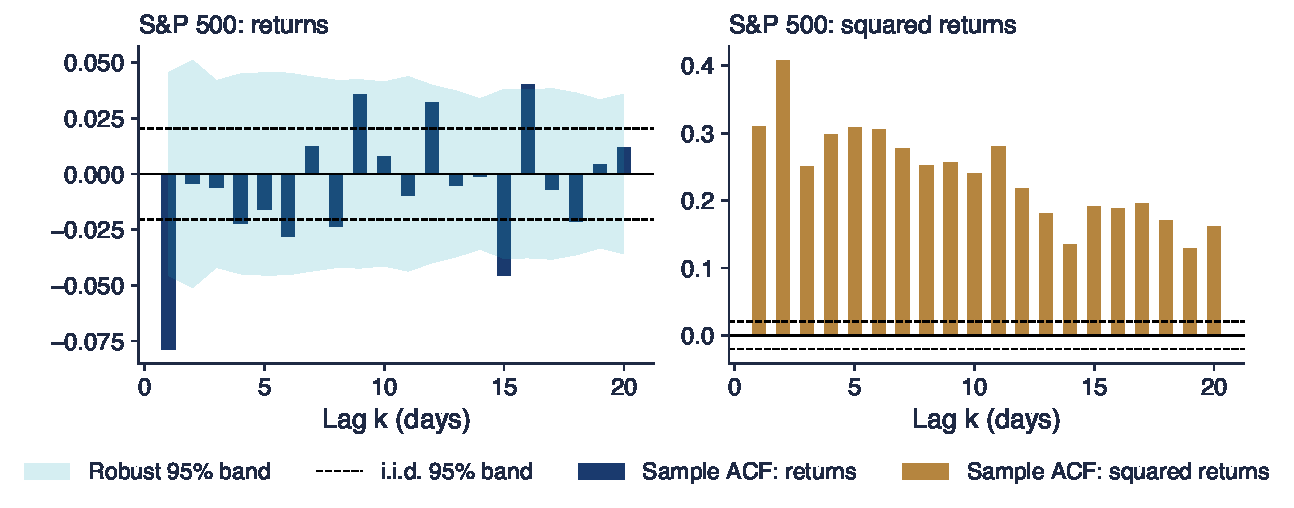
\includegraphics[width=0.96\textwidth,height=0.36\textheight,keepaspectratio]{ch7_sem_b1.pdf}
\end{center}
\vspace{-2mm}
\begin{itemize}
    \item $\hat\rho(1..5)$, returns: $-0.079$, $-0.004$, $-0.006$, $-0.022$, $-0.016$; squared: $0.311$, $0.408$, $0.250$, $0.298$, $0.308$; $T = 9\,240$
    \item Returns: $Q_{LB}(10) = 90.8$ (p $<$\,0.001), $\tilde Q(10) = 18.8$ (p = 0.043); squared: $Q_{LB}(10) = 8015$, $\tilde Q(10) = 189.4$ (both p $<$\,0.001)
    \item Interpretation: squared returns reject RW1 and RW2 (volatility clustering); the robust test rejects RW3 only barely, because of a small negative $\hat\rho(1)$: a weak, short-lived reversal
\end{itemize}\sfmquantlet{Ch_07}{SFM_ch7_seminar}
\end{frame}

\begin{frame}{B2: BET, Bitcoin and Two BVB Stocks [Proposed]}
\itemsize{\footnotesize}
\begin{itemize}
\item \textbf{Question}: for which of the BET, Bitcoin, Banca Transilvania and OMV Petrom does the verdict on autocorrelation change between the classic and the robust test? Model: B1.
\item \textbf{Inputs}: BET since 1997, Bitcoin since 2014, TLV and SNP since 2010 (TLV without 30--31 May 2016), daily log returns in \%
\item \textbf{Tasks}
\begin{enumerate}
    \item Compute $\hat\rho(1)$, $Q_{LB}(10)$ and $\tilde Q(10)$ with p-values for each series.
    \item Compute the runs test $z$ and its p-value for each series.
    \item Mark the series for which the classic and the robust test disagree at 5\%.
    \item Interpretation: why is the BET different from the other three?
\end{enumerate}
\item \textbf{Report}: one table and two sentences
\item Notebook: section B2
\end{itemize}
\end{frame}

\ifsolutions
\begin{frame}{B2: Solution [Proposed]}
\itemsize{\footnotesize}
\begin{center}
\footnotesize
\begin{tabular}{lrrrrrrrr}
\toprule
& $T$ & $\hat\rho(1)$ & $Q_{LB}(10)$ & p & $\tilde Q(10)$ & p & runs $z$ & p \\
\midrule
BET & 7\,243 & ${0.156}$ & $198.3$ & $<$\,0.001 & $42.9$ & $<$\,0.001 & ${-7.75}$ & $<$\,0.001 \\
Bitcoin & 4\,384 & ${-0.022}$ & $20.2$ & 0.028 & $11.9$ & 0.294 & ${2.68}$ & 0.007 \\
TLV & 3\,788 & ${0.010}$ & $29.1$ & 0.001 & $13.2$ & 0.210 & ${-1.68}$ & 0.093 \\
SNP & 3\,815 & ${-0.015}$ & $20.7$ & 0.023 & $9.9$ & 0.446 & ${1.72}$ & 0.085 \\
\bottomrule
\end{tabular}
\end{center}
\begin{itemize}
    \item Classic LB rejects for all four; the robust test only for the BET: the verdict changes for Bitcoin, TLV and SNP
    \item Runs: the BET has far too few runs ($z = -7.75$); Bitcoin has too many ($z = 2.68$): signs alternate slightly more than under independence
    \item Interpretation: the BET is an index of stocks with uneven trading: stale closing prices create positive autocorrelation (thin trading); the single stocks and Bitcoin do not show it
\end{itemize}\sfmquantlet{Ch_07}{SFM_ch7_seminar}
\end{frame}
\fi

\begin{frame}{B3: Unit Roots in the DAX [Solved]}
\itemsize{\footnotesize}
\begin{itemize}
\item \textbf{Question}: what is the order of integration of the DAX log price and of its returns?
\item \textbf{Inputs}: DAX closes since 1990; log price and daily log returns
\item \textbf{Tasks}
\begin{enumerate}
    \item Draw the log price with a fitted linear trend, and the returns.
    \item Run ADF (lag order by AIC), PP and KPSS on the log price with a constant and a trend.
    \item Run the same three tests on the returns with a constant.
    \item Interpretation: does a unit root in the DAX price prove that the DAX is weak-form efficient?
\end{enumerate}
\item \textbf{Report}: the chart, six statistics with p-values and two sentences
\item Notebook: section B3
\end{itemize}
\end{frame}

\begin{frame}{B3: Solution [Solved]}
\itemsize{\scriptsize}
\begin{center}
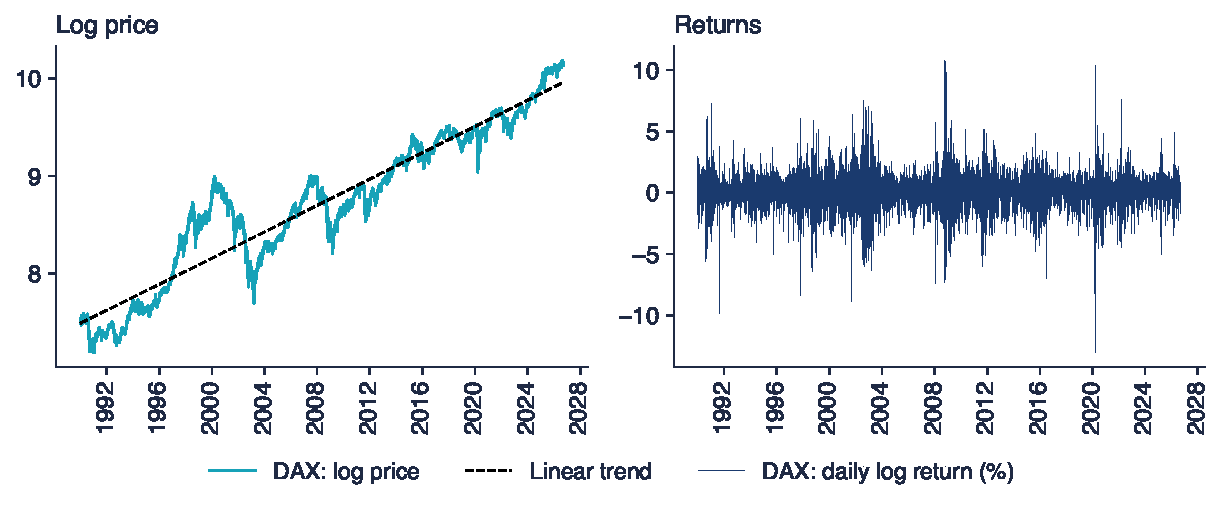
\includegraphics[width=0.96\textwidth,height=0.36\textheight,keepaspectratio]{ch7_sem_b3.pdf}
\end{center}
\vspace{-2mm}
\begin{center}
\scriptsize
\begin{tabular}{lrrr}
\toprule
& ADF & PP & KPSS \\
\midrule
log price (trend) & $-2.69$ (p = 0.239) & $-2.65$ (p = 0.260) & $0.94$ (p $<$\,0.01) \\
returns (constant) & $-23.30$ (p $<$\,0.001) & $-97.40$ (p $<$\,0.001) & $0.04$ (p $>$\,0.10) \\
\bottomrule
\end{tabular}
\end{center}
\begin{itemize}
    \item ADF used 30 lags for the price (AIC); PP and KPSS use 38 Bartlett lags; $T = 9\,288$
    \item Price: no rejection by ADF or PP, rejection by KPSS: $I(1)$; returns: the opposite: $I(0)$
    \item Interpretation: no; a unit root is necessary for a random walk but allows predictable increments; efficiency is tested on the returns (B1, B5)
\end{itemize}\sfmquantlet{Ch_07}{SFM_ch7_seminar}
\end{frame}

\begin{frame}{B4: BET, Bitcoin and TLV [Proposed]}
\itemsize{\footnotesize}
\begin{itemize}
\item \textbf{Question}: do the three unit-root tests agree for the BET, Bitcoin and Banca Transilvania? Model: B3.
\item \textbf{Inputs}: BET since 1997, Bitcoin since 2014, TLV since 2010 (without 30--31 May 2016)
\item \textbf{Tasks}
\begin{enumerate}
    \item Run ADF, PP and KPSS on each log price (constant and trend) and on each return series (constant).
    \item Classify each series as $I(1)$, $I(0)$ or inconclusive.
    \item For an inconclusive case, propose one check that could settle it.
    \item Interpretation: would you trade a ``mean-reverting'' TLV price on this evidence?
\end{enumerate}
\item \textbf{Report}: one table, three classifications and two sentences
\item Notebook: section B4
\end{itemize}
\end{frame}

\ifsolutions
\begin{frame}{B4: Solution [Proposed]}
\itemsize{\footnotesize}
\begin{center}
\scriptsize
\begin{tabular}{lrrrrrr}
\toprule
& ADF price (p) & PP price (p) & KPSS price (p) & ADF ret. & PP ret. & KPSS ret. (p) \\
\midrule
BET & ${-1.73}$ (0.736) & ${-1.54}$ (0.814) & $2.30$ ($<$\,0.01) & ${-13.65}$ & ${-74.47}$ & $0.12$ ($>$\,0.10) \\
Bitcoin & ${-1.48}$ (0.837) & ${-1.54}$ (0.817) & $1.81$ ($<$\,0.01) & ${-20.16}$ & ${-67.84}$ & $0.13$ ($>$\,0.10) \\
TLV & ${-3.46}$ (0.044) & ${-3.35}$ (0.058) & $0.57$ ($<$\,0.01) & ${-12.96}$ & ${-60.79}$ & $0.23$ ($>$\,0.10) \\
\bottomrule
\end{tabular}
\end{center}
\begin{itemize}
    \item BET and Bitcoin: log price $I(1)$, returns $I(0)$
    \item TLV price: ADF rejects at 5\% (p = 0.044), PP does not (p = 0.058), KPSS rejects stationarity: inconclusive; check: test for a structural break, or split the sample
    \item Interpretation: no; a borderline p-value, contradicted by two other tests, on one of many series tested, is not a trading signal
\end{itemize}\sfmquantlet{Ch_07}{SFM_ch7_seminar}
\end{frame}
\fi

\begin{frame}{B5: Variance Ratios of the S\&P 500 [Solved]}
\itemsize{\footnotesize}
\begin{itemize}
\item \textbf{Question}: is the S\&P 500 mean-reverting over horizons of 2 to 20 days, once volatility clustering is taken into account?
\item \textbf{Inputs}: S\&P 500 closes since 1990, daily log returns in \%
\item \textbf{Tasks}
\begin{enumerate}
    \item Compute VR($q$), $Z(q)$ and $Z^*(q)$ for $q = 2, 5, 10, 20$.
    \item Compute the Chow--Denning statistic and compare it with its 5\% critical value.
    \item Draw VR($q$) for $q = 2, \dots, 40$ with the i.i.d.\ and the robust 95\% bands.
    \item Interpretation: is the mean reversion large enough to matter for an investor?
\end{enumerate}
\item \textbf{Report}: a table of twelve numbers, one statistic, the chart and two sentences
\item Notebook: section B5
\end{itemize}
\end{frame}

\begin{frame}{B5: Solution [Solved]}
\itemsize{\scriptsize}
\begin{center}
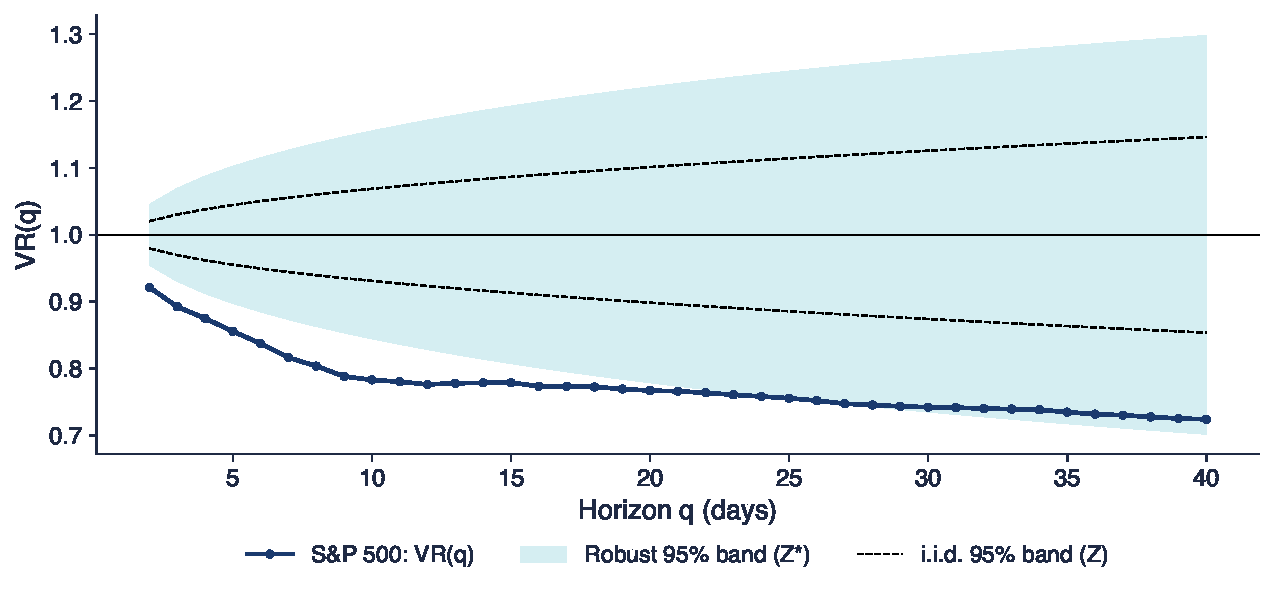
\includegraphics[width=0.96\textwidth,height=0.32\textheight,keepaspectratio]{ch7_sem_b5.pdf}
\end{center}
\vspace{-2mm}
\begin{center}
\scriptsize
\begin{tabular}{lrrrr}
\toprule
& $q = 2$ & $q = 5$ & $q = 10$ & $q = 20$ \\
\midrule
VR($q$) & $0.922$ & $0.856$ & $0.783$ & $0.767$ \\
$Z(q)$ & ${-7.54}$ & ${-6.33}$ & ${-6.17}$ & ${-4.50}$ \\
$Z^*(q)$ & ${-3.37}$ & ${-2.76}$ & ${-2.73}$ & ${-2.06}$ \\
\bottomrule
\end{tabular}
\end{center}
\begin{itemize}
    \item $T = 9\,240$; Chow--Denning: $\max|Z^*| = 3.37 > 2.49$ (p = 0.003): reject the random walk
    \item $Z(2)$ is about 2.2 times $Z^*(2)$: ignoring volatility clustering exaggerates the evidence
    \item Interpretation: significant, but small: the weekly variance is about 86\% of five daily variances; after trading costs this is hardly a profit
\end{itemize}\sfmquantlet{Ch_07}{SFM_ch7_seminar}
\end{frame}

\begin{frame}{B6: Five Emerging Markets [Proposed]}
\itemsize{\footnotesize}
\begin{itemize}
\item \textbf{Question}: which of the WIG20, BUX, PX, BET and BIST 100 departs from a random walk over the last ten years? Model: B5.
\item \textbf{Inputs}: daily log returns from 19 September 2016 to 18 September 2026
\item \textbf{Tasks}
\begin{enumerate}
    \item Compute VR(5), $Z^*(5)$ and its p-value for each market.
    \item Compute the Chow--Denning p-value ($q = 2, 5, 10, 20$) and the automatic VR test with its wild-bootstrap p-value.
    \item Compute the Šidák critical value for five markets tested together at 5\%.
    \item Interpretation: which markets would you call inefficient once you account for testing five markets?
\end{enumerate}
\item \textbf{Report}: one table, one critical value and two sentences
\item Notebook: section B6
\end{itemize}
\end{frame}

\ifsolutions
\begin{frame}{B6: Solution [Proposed]}
\itemsize{\footnotesize}
\begin{center}
\footnotesize
\begin{tabular}{lrrrrrrr}
\toprule
& $T$ & VR(5) & $Z^*(5)$ & p & CD p & automatic VR & p (bootstrap) \\
\midrule
WIG20 & 2\,498 & $0.979$ & ${-0.27}$ & 0.789 & 0.938 & ${-1.09}$ & 0.342 \\
BUX & 2\,492 & $1.033$ & ${0.33}$ & 0.739 & 0.995 & ${0.01}$ & 0.992 \\
PX & 2\,504 & $1.206$ & ${2.08}$ & 0.038 & 0.142 & ${2.56}$ & 0.104 \\
BET & 2\,492 & $1.200$ & ${2.03}$ & 0.042 & 0.159 & ${3.76}$ & 0.034 \\
BIST 100 & 2\,507 & $1.086$ & ${1.34}$ & 0.180 & 0.549 & ${0.04}$ & 0.868 \\
\bottomrule
\end{tabular}
\end{center}
\begin{itemize}
    \item Šidák: each test at $1 - 0.95^{1/5} = 1.02\%$, critical value $2.57$; with five independent tests at 5\%, the chance of at least one false rejection is 22.6\%
    \item PX and BET: $Z^*(5)$ just above 1.96, below $2.57$; Chow--Denning does not reject; only the automatic VR rejects for the BET
    \item Interpretation: no market is clearly inefficient; the BET shows weak, test-dependent momentum
\end{itemize}\sfmquantlet{Ch_07}{SFM_ch7_seminar}
\end{frame}
\fi


%=============================================================================
\section{Part C: Open Questions and AI Critique}
%=============================================================================

\begin{frame}{C1: Has the BET Become More Efficient? [Proposed]}
\itemsize{\footnotesize}
\begin{itemize}
\item \textbf{Question}: how has the predictability of the BET evolved since 1997, including around the FTSE Russell upgrade of September 2020?
\item \textbf{Inputs}: BET daily log returns since 1997; models: B1, B5
\item \textbf{Tasks}
\begin{enumerate}
    \item Compute VR(5) and $Z^*(5)$ on rolling windows of 500 days, one every 21 days, and the share of windows with $|Z^*(5)| > 1.96$ in the first and in the last five years.
    \item Compute $\hat\rho(1)$, VR(5), $Z^*(5)$ and the Chow--Denning p-value in 1997--2006, 2007--2016 and 2017--2026.
    \item Compare VR(5) in the five years before and after 21 September 2020.
    \item List what else changed in the Romanian market at the same time.
    \item Interpretation: how would you separate these changes from the effect of the upgrade?
\end{enumerate}
\item \textbf{Report}: a table, one chart and a plan for a project
\item Notebook: section C1
\end{itemize}
\end{frame}

\ifsolutions
\begin{frame}{C1: Reference Analysis [Proposed]}
\itemsize{\footnotesize}
\begin{center}
\footnotesize
\begin{tabular}{lrrrrr}
\toprule
Period & $T$ & $\hat\rho(1)$ & VR(5) & $Z^*(5)$ & CD p \\
\midrule
1997--2006 & 2306 & $0.270$ & $1.50$ & $6.15$ & $<$\,0.001 \\
2007--2016 & 2516 & $0.066$ & $1.08$ & $0.82$ & 0.262 \\
2017--2026 & 2421 & $0.064$ & $1.20$ & $2.04$ & 0.154 \\
\bottomrule
\end{tabular}
\end{center}
\begin{itemize}
    \item Rolling windows rejecting at 5\%: 89\% in the first five years, 15\% in the last five years
    \item Five years before and after the upgrade: VR(5) $1.12$ ($Z^* = 0.80$) and $1.18$ ($Z^* = 1.78$); difference $z = 0.34$: no evidence
    \item Confounders: COVID-19 (2020), Hidroelectrica listing (2023), volumes, index composition; designs: the same test on BVB stocks, WIG20 and BUX as controls
\end{itemize}\sfmquantlet{Ch_07}{SFM_ch7_seminar}
\end{frame}
\fi

\begin{frame}{C2: Audit an AI Answer [Proposed]}
\itemsize{\scriptsize}
\begin{itemize}
    \item A student asked an AI assistant whether the DAX (daily, since 1990) is weak-form efficient. The answer:
    \item \aiprompt{(a) ADF on the DAX log price gives tau = -2.69, p = 0.24: the unit root is not rejected, so the DAX is weak-form efficient.}
    \item \aiprompt{(b) Ljung-Box Q(10) = 21.83, p = 0.016: DAX returns are predictable, so the DAX is not efficient.}
    \item \aiprompt{(c) For squared returns Q(10) = 3747: DAX returns are not a martingale.}
    \item \aiprompt{(d) VR(10) = 0.93 < 1 shows positive autocorrelation (momentum) in the DAX.}
    \item \aiprompt{(e) Under RW1, VR(q) = 1 at every horizon and the variance of q-day returns is q times the daily variance.}
    \item Tasks
    \begin{itemize}
        \item 1. For each statement, say whether it is correct; if not, give the correct statement and, where possible, the correct number from the notebook (section C2).
        \item 2. Report: a list of five verdicts with one line of justification each.
    \end{itemize}
\end{itemize}
\end{frame}

\ifsolutions
\begin{frame}{C2: Solution [Proposed]}
\itemsize{\footnotesize}
\begin{itemize}
    \item (a) Wrong: a unit root is necessary, not sufficient; $I(1)$ prices can have predictable increments; test the returns
    \item (b) Wrong: $Q_{LB}$ assumes i.i.d.\ returns; the robust $\tilde Q(10) = 8.59$ (p = 0.571) does not reject
    \item (c) Wrong: correlated squared returns are volatility clustering; they reject RW1 and RW2, not the martingale (the robust $\tilde Q$ of the squares, $334.3$, leads to the same conclusion)
    \item (d) Wrong: VR $< 1$ means negative autocorrelation (mean reversion), and $Z^*(10) = -1.21$ is not significant ($Z(10) = -1.95$)
    \item (e) Correct: $\mathrm{Var}(r_t(q)) = q\sigma^2$ under RW1 (indeed under RW3 as well)
\end{itemize}\sfmquantlet{Ch_07}{SFM_ch7_seminar}
\end{frame}
\fi


%=============================================================================
\section{Wrap-Up}
%=============================================================================

\begin{frame}{What You Should Take from Today}
\itemsize{\small}
\begin{itemize}
    \item A unit root in prices is the starting point, not the answer: efficiency is about the returns
    \item Test the martingale with robust statistics ($\tilde Q$, $Z^*$): classic tests mistake volatility clustering for predictability
    \item VR $> 1$: momentum; VR $< 1$: mean reversion; the S\&P 500 reverts slightly, the old BET trended
    \item Many horizons or many markets: use Chow--Denning or a Šidák correction
    \item An AI answer is a draft: check the null of each test, the sign of VR $- 1$ and the robust version
\end{itemize}
\end{frame}

\begin{frame}{After the Seminar}
\itemsize{\small}
\begin{itemize}
    \item Lecture 7 develops each topic of today: efficiency, random walks, ACF tests, unit roots, variance ratios, adaptive markets
    \item Try the [Proposed] tasks in the notebook; the solutions are discussed in class
    \item C1 can grow into a team project: BET stocks, WIG20 and BUX as controls, a block bootstrap of the difference
    \item Reading: \refFHH, Ch.~11; exercises in \refBHL, Ch.~11; \refCLM, Ch.~2
\end{itemize}
\end{frame}


%=============================================================================
\section{References}
%=============================================================================

\begin{frame}{References}
\itemsize{\tiny}
\begin{itemize}
    \item Borak, S., Härdle, W.K., López-Cabrera, B. (2013). \href{https://doi.org/10.1007/978-3-642-33929-5}{\textit{Statistics of Financial Markets: Exercises and Solutions}}, 2nd ed. Springer.
    \item Box, G.E.P., Pierce, D.A. (1970). \href{https://doi.org/10.1080/01621459.1970.10481180}{Distribution of residual autocorrelations in autoregressive-integrated moving average time series models}. \textit{Journal of the American Statistical Association}, 65(332), 1509--1526.
    \item Campbell, J.Y., Lo, A.W., MacKinlay, A.C. (1997). \href{https://doi.org/10.1515/9781400830213}{\textit{The Econometrics of Financial Markets}}. Princeton University Press.
    \item Choi, I. (1999). \href{https://doi.org/10.1002/(SICI)1099-1255(199905/06)14:3<293::AID-JAE503>3.0.CO;2-5}{Testing the random walk hypothesis for real exchange rates}. \textit{Journal of Applied Econometrics}, 14(3), 293--308.
    \item Chow, K.V., Denning, K.C. (1993). \href{https://doi.org/10.1016/0304-4076(93)90051-6}{A simple multiple variance ratio test}. \textit{Journal of Econometrics}, 58(3), 385--401.
    \item Dickey, D.A., Fuller, W.A. (1979). \href{https://doi.org/10.1080/01621459.1979.10482531}{Distribution of the estimators for autoregressive time series with a unit root}. \textit{Journal of the American Statistical Association}, 74(366), 427--431.
    \item Escanciano, J.C., Lobato, I.N. (2009). \href{https://doi.org/10.1016/j.jeconom.2009.03.001}{An automatic Portmanteau test for serial correlation}. \textit{Journal of Econometrics}, 151(2), 140--149.
    \item Fama, E.F. (1970). \href{https://doi.org/10.1111/j.1540-6261.1970.tb00518.x}{Efficient capital markets: a review of theory and empirical work}. \textit{Journal of Finance}, 25(2), 383--417.
    \item Franke, J., Härdle, W.K., Hafner, C.M. (2019). \href{https://doi.org/10.1007/978-3-030-13751-9}{\textit{Statistics of Financial Markets: An Introduction}}, 5th ed. Springer.
    \item Kim, J.H. (2009). \href{https://doi.org/10.1016/j.frl.2009.04.003}{Automatic variance ratio test under conditional heteroskedasticity}. \textit{Finance Research Letters}, 6(3), 179--185.
    \item Kwiatkowski, D., Phillips, P.C.B., Schmidt, P., Shin, Y. (1992). \href{https://doi.org/10.1016/0304-4076(92)90104-Y}{Testing the null hypothesis of stationarity against the alternative of a unit root}. \textit{Journal of Econometrics}, 54(1--3), 159--178.
    \item Ljung, G.M., Box, G.E.P. (1978). \href{https://doi.org/10.1093/biomet/65.2.297}{On a measure of lack of fit in time series models}. \textit{Biometrika}, 65(2), 297--303.
    \item Lo, A.W., MacKinlay, A.C. (1988). \href{https://doi.org/10.1093/rfs/1.1.41}{Stock market prices do not follow random walks: evidence from a simple specification test}. \textit{Review of Financial Studies}, 1(1), 41--66.
    \item MacKinnon, J.G. (1996). \href{https://doi.org/10.1002/(SICI)1099-1255(199611)11:6<601::AID-JAE417>3.0.CO;2-T}{Numerical distribution functions for unit root and cointegration tests}. \textit{Journal of Applied Econometrics}, 11(6), 601--618.
    \item Phillips, P.C.B., Perron, P. (1988). \href{https://doi.org/10.1093/biomet/75.2.335}{Testing for a unit root in time series regression}. \textit{Biometrika}, 75(2), 335--346.
    \item Said, S.E., Dickey, D.A. (1984). \href{https://doi.org/10.1093/biomet/71.3.599}{Testing for unit roots in autoregressive-moving average models of unknown order}. \textit{Biometrika}, 71(3), 599--607.
    \item Wald, A., Wolfowitz, J. (1940). \href{https://doi.org/10.1214/aoms/1177731909}{On a test whether two samples are from the same population}. \textit{Annals of Mathematical Statistics}, 11(2), 147--162.
\end{itemize}
\end{frame}

\end{document}
